\chapter{Simulation Engine for DT-based Dynamic Mirroring}\label{ch:ch3}

The digital twin approach incorporates three important parts: physical system, virtual system, and the data exchange between these two systems. The first step in establishing a DT is building accurate models of the real system or asset, which can mirror the behavior of the real twin. To establish the virtual model, the best available knowledge of system dynamics should be used and integrated with the available data \autocite{jrn_bazmohammadi_2022}. 

In order to dynamically mirror the PEDGs, the DT must consider the transient behavior of major components of the power system. Among such components are distributed generators, electrical energy storage systems, transmission lines, loads, transformers, busbars and terminals. By incorporating rigorous dynamic DT models into these components within injection of real-time data, we can obtain a dynamic representation of the whole system \autocite{10938101}. The dynamic interaction of these components can be described by means of differential and algebraic equations, which are summarized in a DAE system:

\begin{equation}
    \begin{array}{l}
\dot{\boldsymbol{x}}=\boldsymbol{f}(\boldsymbol{x}(t), \boldsymbol{z}(t), \boldsymbol{u}(t), \boldsymbol{p}), \\
0=\boldsymbol{g}(\boldsymbol{x}(t), \boldsymbol{z}(t), \boldsymbol{u}(t), \boldsymbol{p}), \\
\boldsymbol{y}(t)=\boldsymbol{h}(\boldsymbol{x}(t), \boldsymbol{z}(t), \boldsymbol{u}(t), \boldsymbol{p}).
\end{array}
\end{equation}

Whereas the vector $\boldsymbol{x} \in \mathbb{R}^{\mathrm{n}}$ denotes the differential states, the vector $\boldsymbol{z} \in \mathbb{R}^{\mathrm{n}}$ represents the algebraic states, $\boldsymbol{u} \in \mathbb{R}^{\mathrm{n}}$ describes the control inputs, $\boldsymbol{y} \in \mathbb{R}^{\mathrm{n}}$ represents the measurable outputs and $\boldsymbol{p} \in \mathbb{R}^{\mathrm{n}}$ comprises all parameters.  Functions $\boldsymbol{f}, \boldsymbol{g}$, and $\boldsymbol{h}$ describe these states and system responses.

Modeling an interconnected power system involves assembling separate sets of equations that represent the behavior of individual components and equipment. These equipment models, which include sub-models like controllers (e.g., PLL, current, voltage, droop), are interconnected by assigning the output of one model as the input for another. Additional system elements, such as reactive power compensation devices, converters, or various power plant models should be included. Figure~\cref{fig:ps_structure} illustrates this arrangement, depicting the interconnected system as a collection of composite sub-models.

\begin{figure}[htbp]
    \centering
    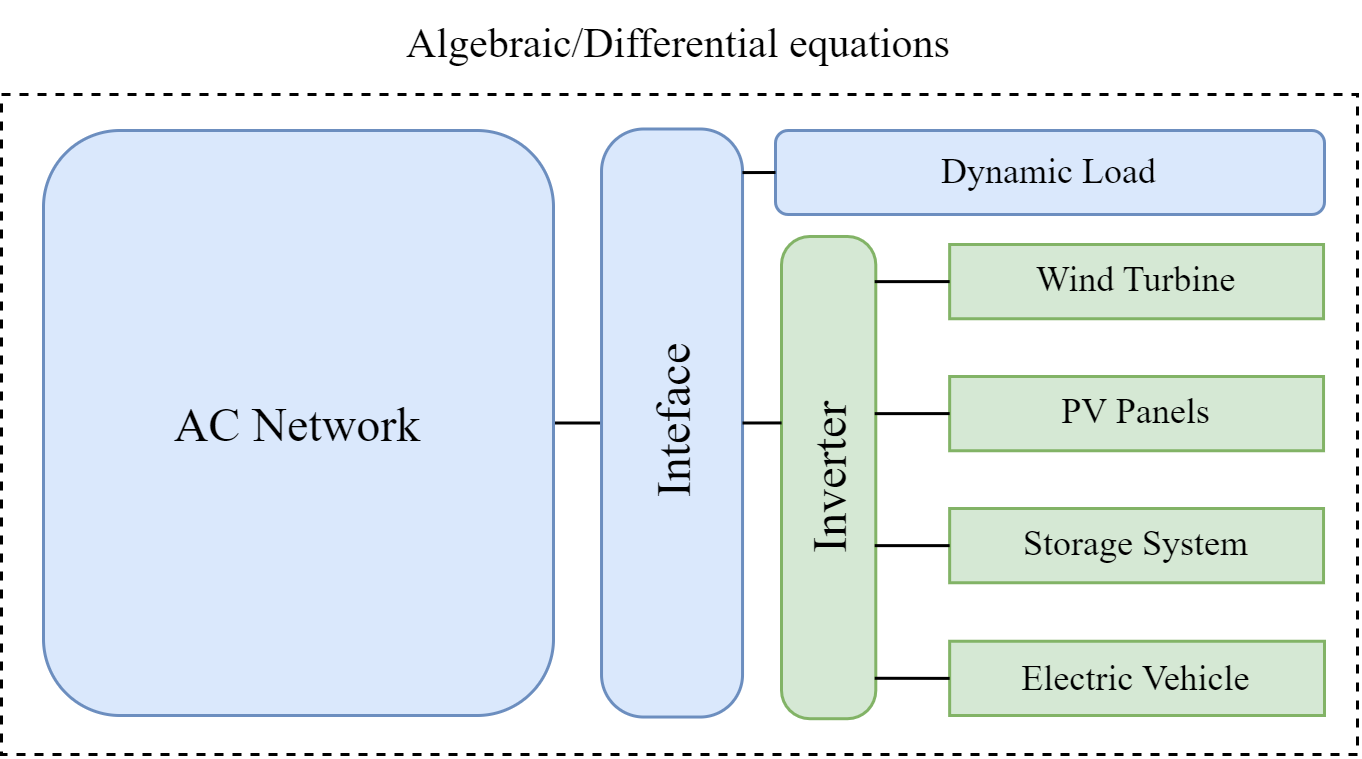
\includegraphics[width = 1\columnwidth]{ps_structure_2.png}
    \caption{Simplified microgrid structure with distributed energy resources.}
    \label{fig:ps_structure}
\end{figure}

\section{Vanadium Redox Flow Battery}\label{sec:ch3/sec1}

A digital twin for vanadium redox flow batteries (VRFBs) offers a powerful framework for real-time, dynamic state monitoring, enabling predictive insights and optimized operation of these large-scale energy storage systems \autocite{10615087}. By creating a high-fidelity virtual replica of the physical battery, the digital twin continuously processes operational data, such as electrolyte flow rates, cell voltages, and temperature profiles, and integrates them with advanced electrochemical models to estimate internal states that are otherwise difficult to measure directly \autocite{Pugach2020, bogdanov_dynamic_2023}. This approach allows operators to detect performance deviations early, forecast SOC and SOH trends, and implement data-driven control strategies to extend battery lifespan and improve efficiency. In this chapter, the DT of VRFB are presented for real-time accurate SOC and output voltage observing.  

To create a digital twin of a VRFB system, it is necessary to consider the the dynamics of main system components that can demonstrate nonlinear behavior at some operating conditions. The good candidate for that is zero dimensional dynamic model that is an  optimal trade off between the complexity and accuracy \autocite{pugach_zero_2018}.

% \subsection{Model Formulation}

In Figure~\cref{fig:vrfb_st}, the traditional configuration of the VRFB system is illustrated.
 \begin{figure}[t]
    \centering
    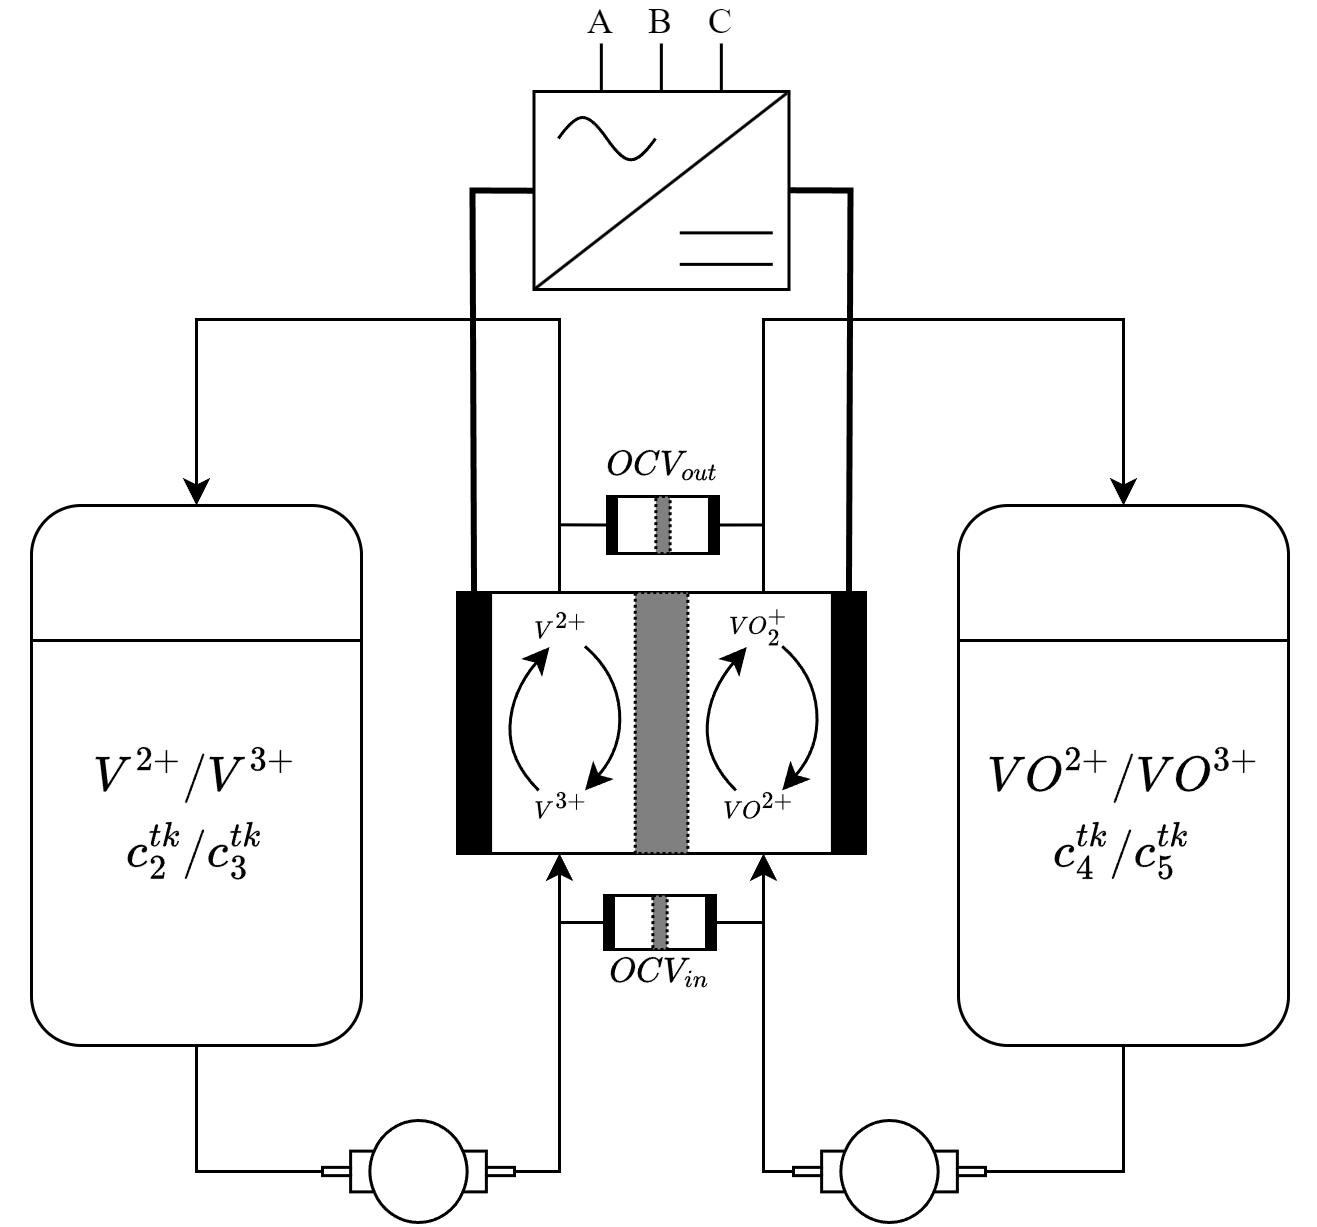
\includegraphics[width = 0.8\columnwidth]{vrfb_diagram.png}
    \caption{A diagram of the VRFB storage system equipped with inlet and outlet open circuit cells.}
    \label{fig:vrfb_st}
    % \vspace*{-0.3cm}
\end{figure}
Vanadium electrolytes contained in two separate tanks with a volume $V_{tk}$ store electrical energy. Via redox reactions electrochemical energy conversions occur in a stack of cells, through which the electrolytes are circulated from the tanks. It's involving the various vanadium $V^{2+}/V^{3+}$ and $V^{4+}/V^{5+}$ redox couples \autocite{ng_understanding_2010}:
\begin{equation}
    \label{eq:redox_pos}
        VO^{2+} + H_2O \rightleftharpoons VO^+_2 + 2H^+ + e^-,
\end{equation}
\begin{equation}
    \label{eq:redox_neg}
        V^{3+} + e^- \rightleftharpoons V^{2+}.
\end{equation}

The configuration of the cell involves a pair of half-cells, divided by a membrane to avoid intermixing. However, transmembrane transfer of certain vanadium ions (crossover) may occur, potentially leading to secondary reactions that contribute to self-discharge and nonlinear voltage fluctuations during both charging and discharging operations.
% \autocite{jrn_pugach_2019}.

The total cell voltage $(U_{cell})$ under a specified load can be resolved into two components: the equilibrium potential and internal losses:
% , as indicated in \autocite{jrn_morozov_2024}:
\begin{equation}
    \label{eq:nernst}
        U_{cell} = U_0^* + \dfrac{RT}{F} \ln{ \left[ \left(\dfrac{c_{5}}{c_{4}}\right)\left(\dfrac{c_{2}}{c_{3}}\right) \right] } + U_{loss},
\end{equation}
where $U_0^*$ is the total cell voltage, $c_2,c_3,c_4,c_5$ are the concentrations of vanadium species $V^{2+}/V^{3+}, VO^{2+},VO_{2}^+$, respectively, $R=\SI{8.314}{J/Kmol}$ is the gas constant, $T=\SI{298}{K}$ is the electrolyte temperature, $F=\SI{96485.332}{C/mol}$ is the Faraday constant. Internal losses are cause the change of cell voltage and offered by activation, ohmic, and concentration overvoltages \autocite{pugach_zero_2018}:

\cref{eq:redox_pos,eq:redox_neg,eq:nernst} clearly show that four different vanadium ions ($V^{2+},V^{3+},V^{4+},V^{5+}$) participate in the battery's redox reactions. Therefore, the instantaneous state of the battery is determined by eight concentrations of vanadium ions, four of which are present within the cell, and the remaining four are situated in the storage tank.

Changes in concentrations within the tank and the cell \autocite{pugach_zero_2018} can be captured by the following equation of the mass balance system in compact matrix form:
% \autocite{jrn_pugach_2022}:
\begin{equation}
    \label{eq:mb_dyn}
        \dot{x} = QAx+ \gamma Jx+Dw,
\end{equation}
where the state vector $x \in \mathbb{R}^{8}$ is represented by eight concentrations of the i-th vanadium ion in the tank and the half-cell:
\begin{equation}
    \label{eq:conc_state}
        x = {\left({c_2^{t},c_3^{t},c_4^{t},c_5^{t},c_2^{cell},c_3^{cell},c_4^{cell},c_5^{cell}}\right)}^T,
\end{equation}

Here, the convection flux due to electrolyte pumping is represented by the flow rate $Q$. The crossover matrix $J$ describes the movement of vanadium ions across the membrane. The system is influenced by an applied current that acts as an external disturbance $w$. To precisely model the effect of the crossover flux, a scaling crossover factor $\gamma$ is applied to modify the overall crossover term.
% \autocite{jrn_bogdanov_2023}.
% Here, the flow rate $Q$ characterizes the convection flux arising from electrolyte pumping. The crossover matrix  $J$ encapsulates vanadium ions fluxes across the membrane. The applied current serves as an external disturbance input to the system $w$. For accurate simulation of crossover flux effect, a scaling crossover factor $\gamma$ is introduced as a multiplicative adjustment to overall crossover term, as it was proposed in our previous work \autocite{jrn_bogdanov_2023}. The matrices are:
\begin{equation}
    \begin{gathered}
    \mathcal{A}=\left[\begin{array}{rr}
    -\alpha & \alpha \\
    \beta & -\beta
    \end{array}\right] \otimes \mathbf{I}_4,
    \end{gathered}
\end{equation}
\begin{equation}
    \begin{gathered}
    \mathcal{J}=\left[\begin{array}{ll}
    0 & 0 \\
    0 & 1
    \end{array}\right] \otimes\left[\begin{array}{rrrr}
    -J_2 & 0 & -J_4 & -2 J_5 \\
    0 & -J_3 & 2 J_4 & 3 J_5 \\
    3 J_2 & 2 J_3 & -J_4 & 0 \\
    -2 J_2 & -J_3 & 0 & -J_5
    \end{array}\right], \\
    \end{gathered}
\end{equation}
\begin{equation}
    \begin{gathered}
    \mathcal{D}=\left[\begin{array}{llllll}
    % 0,0,0,0,{1\over{F V_c}},-{1\over{F V_c}},-{1\over{F V_c}},{1\over{F V_c}}
    0,0,0,0,\frac{1}{F V_c},-\frac{1}{F V_c},-\frac{1}{F V_c},\frac{1}{F V_c}
    \end{array}\right]^{\top}.
    \end{gathered}
\end{equation}

Here, $\mathbf{I}_4 \in \mathbb{R}^{4 \times 4}$ denotes the identity matrix, $\alpha=1 / V_{tk}$, $\beta=1 /\left(n_c V_c\right)$. The Kronecker product is represented as $\otimes$. The matrix $J$ signifies the crossover parasitic dynamics, and its elements  $J_2,J_3,J_4,J_5$, which are functions of the current $w$ \autocite{pugach_zero_2018}.

% The stored energy in the tanks at some moment of time $SOC(t)$ is defined as the ratio of the instantaneous stored energy to the maximum allowable value of the stored energy:
The energy that is stored in the tanks at a particular point in time, $SOC(t)$, is determined by dividing the current stored energy by the highest permissible value of the stored energy \autocite{ng_understanding_2010}:
\begin{equation}
    SOC(t) \equiv E_S(t) / E_{s, \max }.
\end{equation}

The battery's maximum stored energy is directly linked to the cumulative concentration of electrochemical redox pairs. Meanwhile, the energy at any given moment is directly related to the amount of active species present.
% Meanwhile, the instantaneous value of energy is proportional to the concentration of the active species.
% ($V^{2+}$ and $VO^{2+}$ ions). 
Moreover, we should take into account the phenomenon of crossover, which leads to a reduction in SOC. Consequently, the estimation of the SOC is based on the minimum value of the aforementioned ratios \autocite{pugach_zero_2018}:
\begin{equation}
    \label{eq:soc_dt}
    SOC(t)=\min \left(\frac{c_2(t)}{\left(c_2(t)+c_3(t)\right)}, \frac{c_5(t)}{c_5(t)+c_4(t)}\right).
\end{equation}


\subsection{Identification of Parameters}\label{subsec:ch3/sec1/sub1}
The DT application relies on zero-dimensional modeling and real-time measurement data to simulate VRFB behavior. However, during long battery cycling, component degradation leads to parameter mismatch of DT model with battery VRFB system. To maintain accuracy, there is a need to identify parameter values of the battery. 

These are related to internal physical and chemical processes that occur during operation, such as the undesired migration of vanadium ions via the membrane, electrode activation, concentration, and ohmic polarizations, and capacity deterioration over time because of uneven vanadium concentrations. For identification of the VRFB system parameters we used the approach proposed in our previous work \autocite{bogdanov_parameter_2023}.

The VRFB model presented above involves the identification of six unknown parameters, including the equivalent overall vanadium concentration $c_b$, the crossover multiplication factor $\gamma$, the formal potential of the cell $U_0^*$, cell resistivity $r_{c e l l}$, the slope $\alpha$ and the growth rate  $\beta$ of the mass transfer coefficient:
\begin{equation}
    \label{eq:idn}
    \xi=\left(c_b, \gamma, r_{c e l l}, U_0^*, \alpha, \beta\right)^T .
\end{equation}

% The ultimate design of the digital twin for the VRFB state of charge estimator is depicted in Figure~\cref{fig:vrfb_dt}. By leveraging digital twin technology, this state estimator acquires and interprets signals related to current, temperature, and flowrate, achieving real-time monitoring of the battery's state. This setup provides for the exhaustive management and surveillance of the VRFB, capitalizing on the advanced features offered by the digital twin.

In the first step, a discharge polarization curve is experimentally measured at a state of charge $S O C_0$ of $50 \%$ and a specified electrolyte flow rate. Under these conditions, the concentrations of the four vanadium ion species are equal, making the logarithmic term in equilibrium potential is equal to zero. The fitting process involves using an explicit voltage–current relationship:
\begin{equation}
    \label{eq:idt_ubat}
    U_{b a t}(I)=N\left(U_0^*-\frac{|I| \cdot A S R}{\Lambda_{e l}}-\frac{2 R T}{F} \ln \left(1-\frac{|I|}{S O C_0 c_0^* \Lambda_{e l} F u^\beta}\right)\right),
\end{equation}
where $c_0^*=\alpha \cdot c_0$. The parameters are estimated using the least squares method by minimizing the sum of squared differences between the experimental measurements and the simulated values:
\begin{equation}
\begin{aligned}
\min_{c_0^*, ASR, U_0^*, \beta} \quad 
& \varepsilon_1(\xi) = \frac{1}{l} \sum_{m=1}^{l} \left(U^{\text{sim}}_{\text{bat}_m}(\xi, I) - U^{\text{exp}}_{\text{bat}_m}(I)\right)^2 \\
\text{subject to} \quad 
& (c_0^*)^{\min} \leq (c_0^*) \leq (c_0^*)^{\max} \\
& ASR^{\min} \leq ASR \leq ASR^{\max} \\
& (U_0^*)^{\min} \leq (U_0^*) \leq (U_0^*)^{\max} \\
& \beta^{\min} \leq \beta \leq \beta^{\max}
\end{aligned}
\end{equation}
where $l$ represents the total number of points on the polarization curve, and the index $m$ refers to each current data point. Then $c_0^*, \beta, A S R$ and $U_0^*$ are fixed for use in the second stage.

In the second step, the charge-discharge curve is obtained under constant load current and a fixed electrolyte flow rate. The optimization problem is then formulated to minimize the squared error between the measured and simulated voltages during the entire cycle:
\begin{equation}
\begin{aligned}
\min_{c_b, \alpha, \gamma} \quad & \varepsilon(\xi) = \frac{1}{n} \sum_{k=1}^{n} \left(U^{\text{sim}}_{\text{bat}k}(\xi) - U^{\text{exp}}_{\text{bat}k}\right)^2 \\
\text{subject to} \quad & c_b^{\min} \leq c_b \leq c_b^{\max} \\
& \alpha^{\min} \leq \alpha \leq \alpha^{\max} \\
& \gamma^{\min} \leq \gamma \leq \gamma^{\max} \\
& c_b \cdot \alpha = c_b^{*}
\end{aligned}
% \tag{4.11}
\end{equation}
where $n$ denotes the number of data points in a complete charge-discharge cycle, and the index $k$ represents each time step. Parameters $\beta, A S R$ and $U_0^*$ are taken as known from the previous stage.  The nonlinear constraint involving $c_0^*$ to obtain the values of $\alpha$ and $c_0$.  Initial parameter values and allowable ranges $\left[\xi^{\text {min }} ; \xi^{\text {max }}\right]$ are taken from literature data and known properties of the experimental setup. Finally, the optimal set of parameters $\xi$ is obtained and used for simulation under other load conditions.

\section{Power Electronic Interface}\label{sec:ch3/sec2}
The typical configuration of Voltage-Sourced Converter (VSC), shown in Figure~\cref{fig:vsc_scheme}, includes a bidirectional converter with both turn-on and turn-off control capability, optionally a transformer and a condenser on the DC side of the converter \autocite{Milano_2019_ess}. 

\begin{figure}[htbp]
    \centering
    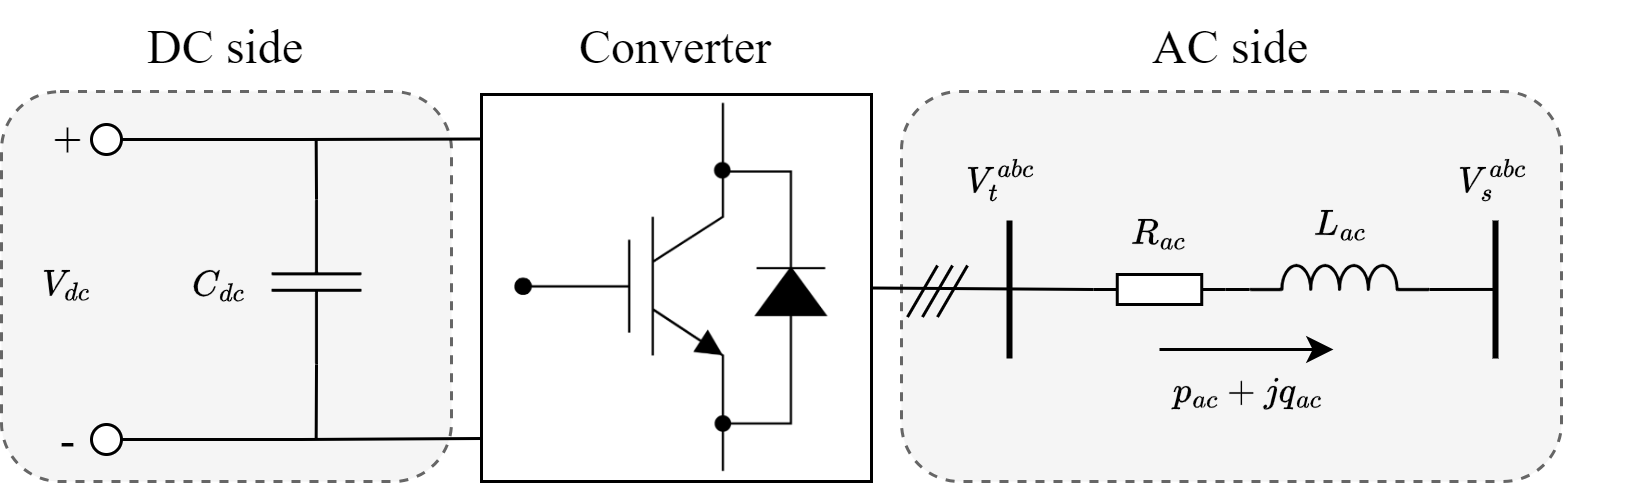
\includegraphics[width = 0.9\columnwidth]{vsc_scheme2.png}
    \caption{Simplified scheme of voltage source converter.}
    \label{fig:vsc_scheme}
\end{figure}

The two-level, three-phase VSC shown in Figure~\cref{fig:2lev_vsc} represents perhaps the most typical configuration among all VSC possibilities. In this setup, each AC terminal is connected to a half-bridge converter, which can assume a voltage of either $v_{\mathrm{dc}} / 2$ or $-v_{\mathrm{dc}} / 2$, where $v_{\mathrm{dc}}$ denotes the DC-side voltage of the converter. Each half-bridge converter consists of two fully controllable reverse-conducting switch cells, each made up of a transistor $\mathrm{T}_i$ and an antiparallel diode $\mathrm{D}_i$ (where $i=1,2,\ldots,6$). Typical examples of such switches include the integrated gate bipolar transistor and the integrated gate-commutated thyristor.

\begin{figure}[htbp]
    \centering
    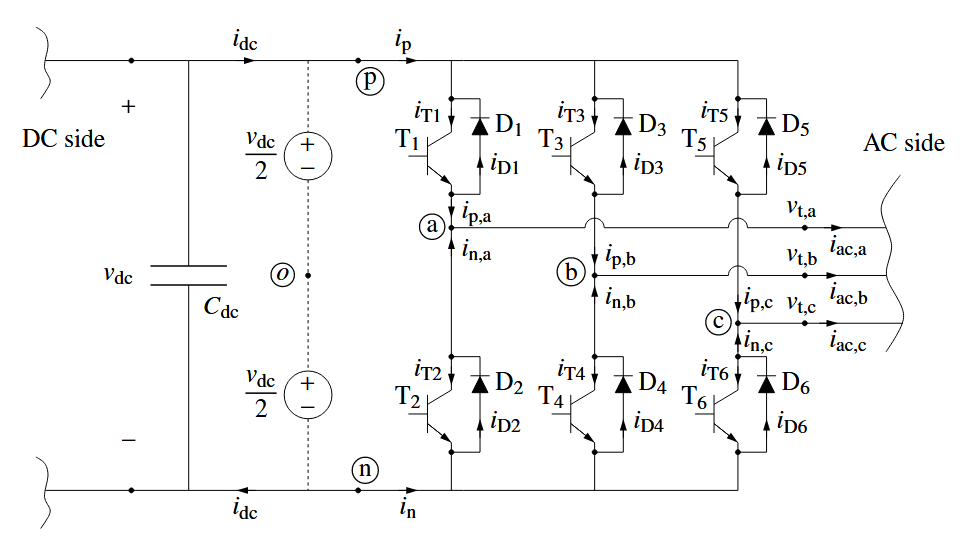
\includegraphics[width = 0.85\columnwidth]{2lev_vsc.png}
    \caption{Ideal two-level three-phase VSC diagram.}
    \label{fig:2lev_vsc}
\end{figure}

The voltage, $v_{\mathrm{t, abc}}$, on the AC side of the converter is influenced by both $v_{\mathrm{dc}}$ and the switching logic characteristic of $\mathrm{T}_i$, derived via PWM control \autocite{mohan2003power}. PWM works by comparing a high-frequency carrier signal ( $f_{\text {carr }} \sim \mathrm{kHz}$ ), typically of triangular shape ( $[-1,1]$ ), with a lower-frequency modulation signal. In two-level, three-phase VSCs, this modulation signal comprises three-phase balanced sinusoidal functions, meaning $\boldsymbol{v}_{\mathrm{t, abc}}$ has equal amplitudes across its three phases, each separated by a $2 \pi / 3$ rad phase shift \autocite{Milano_2019_ess}.

The switching logic of $\mathrm{T}_1, \mathrm{~T}_3$ and $\mathrm{T}_5$ is as follows:
\begin{equation}
    \begin{aligned}
    k_{\mathrm{T} 1,3,5}(t)= \begin{cases}1, & \text { if the modulating signal exceeds the carrier signal, } \\ 0, & \text { otherwise }\end{cases}
    \end{aligned}
\end{equation}

The states of $\mathrm{T}_2, \mathrm{~T}_4$, and $\mathrm{T}_6$ are inverse to those of $\mathrm{T}_1, \mathrm{~T}_3$, and $\mathrm{T}_5$. Hence,
\begin{equation}
    \begin{aligned}
    k_{\mathrm{T} 1}(t)+k_{\mathrm{T} 2}(t)=k_{\mathrm{T} 3}(t)+k_{\mathrm{T} 4}(t)=k_{\mathrm{T} 5}(t)+k_{\mathrm{T} 6}(t)=1.
    \end{aligned}
\end{equation}

The switch is closed when $k_{\mathrm{T} i}=1$, allowing the AC current $\boldsymbol{i}_{\mathrm{ac}, \mathrm{abc}}$ to flow in required direction.

The switching model can accurately represent the behavior of the ideal VSC. More detailed models of the switches that take into account switching losses, snubber circuits, etc., can be used for an accurate representation of the converter dynamic behavior. Such detailed models show some drawbacks, as follows \autocite{Milano_2019_ess}:
\begin{itemize}
    \item Modeling the dynamics of circuitry and controllers in a switching framework is often challenging. 
    \item In models with large time scales relative to converter switching, high-frequency circuit dynamics are typically ignored.
    \item Transient stability studies with switching models are computationally heavy due to the need for microsecond time steps. 
\end{itemize}

The converter's averaged model addresses these challenges \autocite{sira2006control,middlebrook1976ieee}, by averaging the converter's instantaneous values over a time period typically corresponding to the carrier signal's switching period. In this model, the terminal voltage at the AC side of the VSC can be expressed as a function of the modulating signal, as follows:
\begin{equation}
    \begin{aligned}
        \underline{v}_{\mathrm{t}}^{abc}(t)=\frac{v_{\mathrm{dc}}}{2} \boldsymbol{m}_{\mathrm{abc}}(t)=\frac{v_{\mathrm{dc}}}{2}\left[\begin{array}{l}
        m(t) \cos \left(\omega_{\mathrm{ms}}(t) t+\theta_o\right) \\
        m(t) \cos \left(\omega_{\mathrm{ms}}(t) t+\theta_o-\frac{2 \pi}{3}\right) \\
        m(t) \cos \left(\omega_{\mathrm{ms}}(t) t+\theta_o+\frac{2 \pi}{3}\right)
        \end{array}\right]
    \end{aligned}
\end{equation}
where $m$ denotes the amplitude, $\omega_{\mathrm{ms}}$ represents the frequency of the modulating signal, and $\theta_o$ is the phase offset.

\subsection{Coordinate Transformation}

During the modeling process, three coordinate systems are interrelated to describe dynamic states within the network and control loop: the three-phase, $\alpha \beta$, and $dq$ coordinates. Figure~\cref{fig:coord_transform} illustrates the transformation between these. The Clarke transformation \autocite{6739414} converts the three-phase sinusoidal variables into rotated real and imaginary components. Variables in the $\alpha \beta$-coordinate are expressed as follows:
\begin{equation}
    \begin{aligned}
        \underline{x}(t)=x_a(t)+j \cdot x_\beta(t)
    \end{aligned}
\end{equation}
where $x_\alpha$ and $x_\beta$ denote the real and imaginary components of the state variable $\underline{x}(t)$. The transformation from three-phase to $\alpha \beta$ coordinates employs the general matrix $T_{\mathrm{M}}$.

\begin{equation}
    \begin{aligned}
        \left[\begin{array}{l}
        x_0 \\
        x_{\alpha} \\
        x_{\beta}
        \end{array}\right]=T_{\mathrm{M}} \cdot\left[\begin{array}{l}
        x_{\mathrm{a}} \\
        x_{\mathrm{b}} \\
        x_{\mathrm{c}}
        \end{array}\right]=\frac{1}{3} \cdot\left[\begin{array}{ccc}
        1 & 1 & 1 \\
        2 & -1 & -1 \\
        0 & \sqrt{3} & -\sqrt{3}
        \end{array}\right] \cdot\left[\begin{array}{l}
        x_{\mathrm{a}} \\
        x_{\mathrm{b}} \\
        x_{\mathrm{c}}
        \end{array}\right]
    \end{aligned}
\end{equation}
where the variables $x_\alpha$ and $x_\beta$ are given by
\begin{equation}
    \begin{aligned}
        & x_{\mathrm{a}}=\frac{1}{3}\left(2 \cdot x_{\mathrm{a}}-x_{\mathrm{b}}-x_{\mathrm{c}}\right) \\
        & x_\beta=\frac{1}{3}\left(\sqrt{3} \cdot x_{\mathrm{b}}+\sqrt{3} \cdot x_{\mathrm{c}}\right)
    \end{aligned}
\end{equation}
In a three-phase system, the states $x_{\mathrm{a}}, x_{\mathrm{b}}, x_{\mathrm{c}}$ transform into two main components due to system symmetry, simplifying representation through space vector for both instantaneous and amplitude values. This results in a fully decoupled system. For controller design, converting from stationary three-phase and $\alpha \beta$ coordinates to a rotating system with rotor speed is practical. This system, aligned with the rotor or pole wheel (see Figure~\cref{fig:coord_transform}), benefits from easier representation of electrical dynamics and transforms sinusoidal variables into steady-state form, enabling classical control strategies similar to the well-controlled DC machine. The $\alpha \beta$ to $dq$-coordinate transformation is denoted by

\begin{equation}
    \begin{aligned}
        \left[\begin{array}{l}
        x_{\mathrm{d}} \\
        x_{\mathrm{q}}
        \end{array}\right]=T_{\mathrm{R}} \cdot\left[\begin{array}{l}
        x_\alpha \\
        x_\beta
        \end{array}\right]=\left[\begin{array}{cc}
        \cos \varphi & \sin \varphi \\
        -\sin \varphi & \cos \varphi
        \end{array}\right] \cdot\left[\begin{array}{l}
        x_\alpha \\
        x_\beta
        \end{array}\right]
    \end{aligned}
\end{equation}

where $\varphi=\omega t$ is the angle of the difference between both coordinates. $T_{\mathrm{R}}$ is the transformation matrix for $dq$-coordinate.

\begin{figure}[htbp]
    \centering
    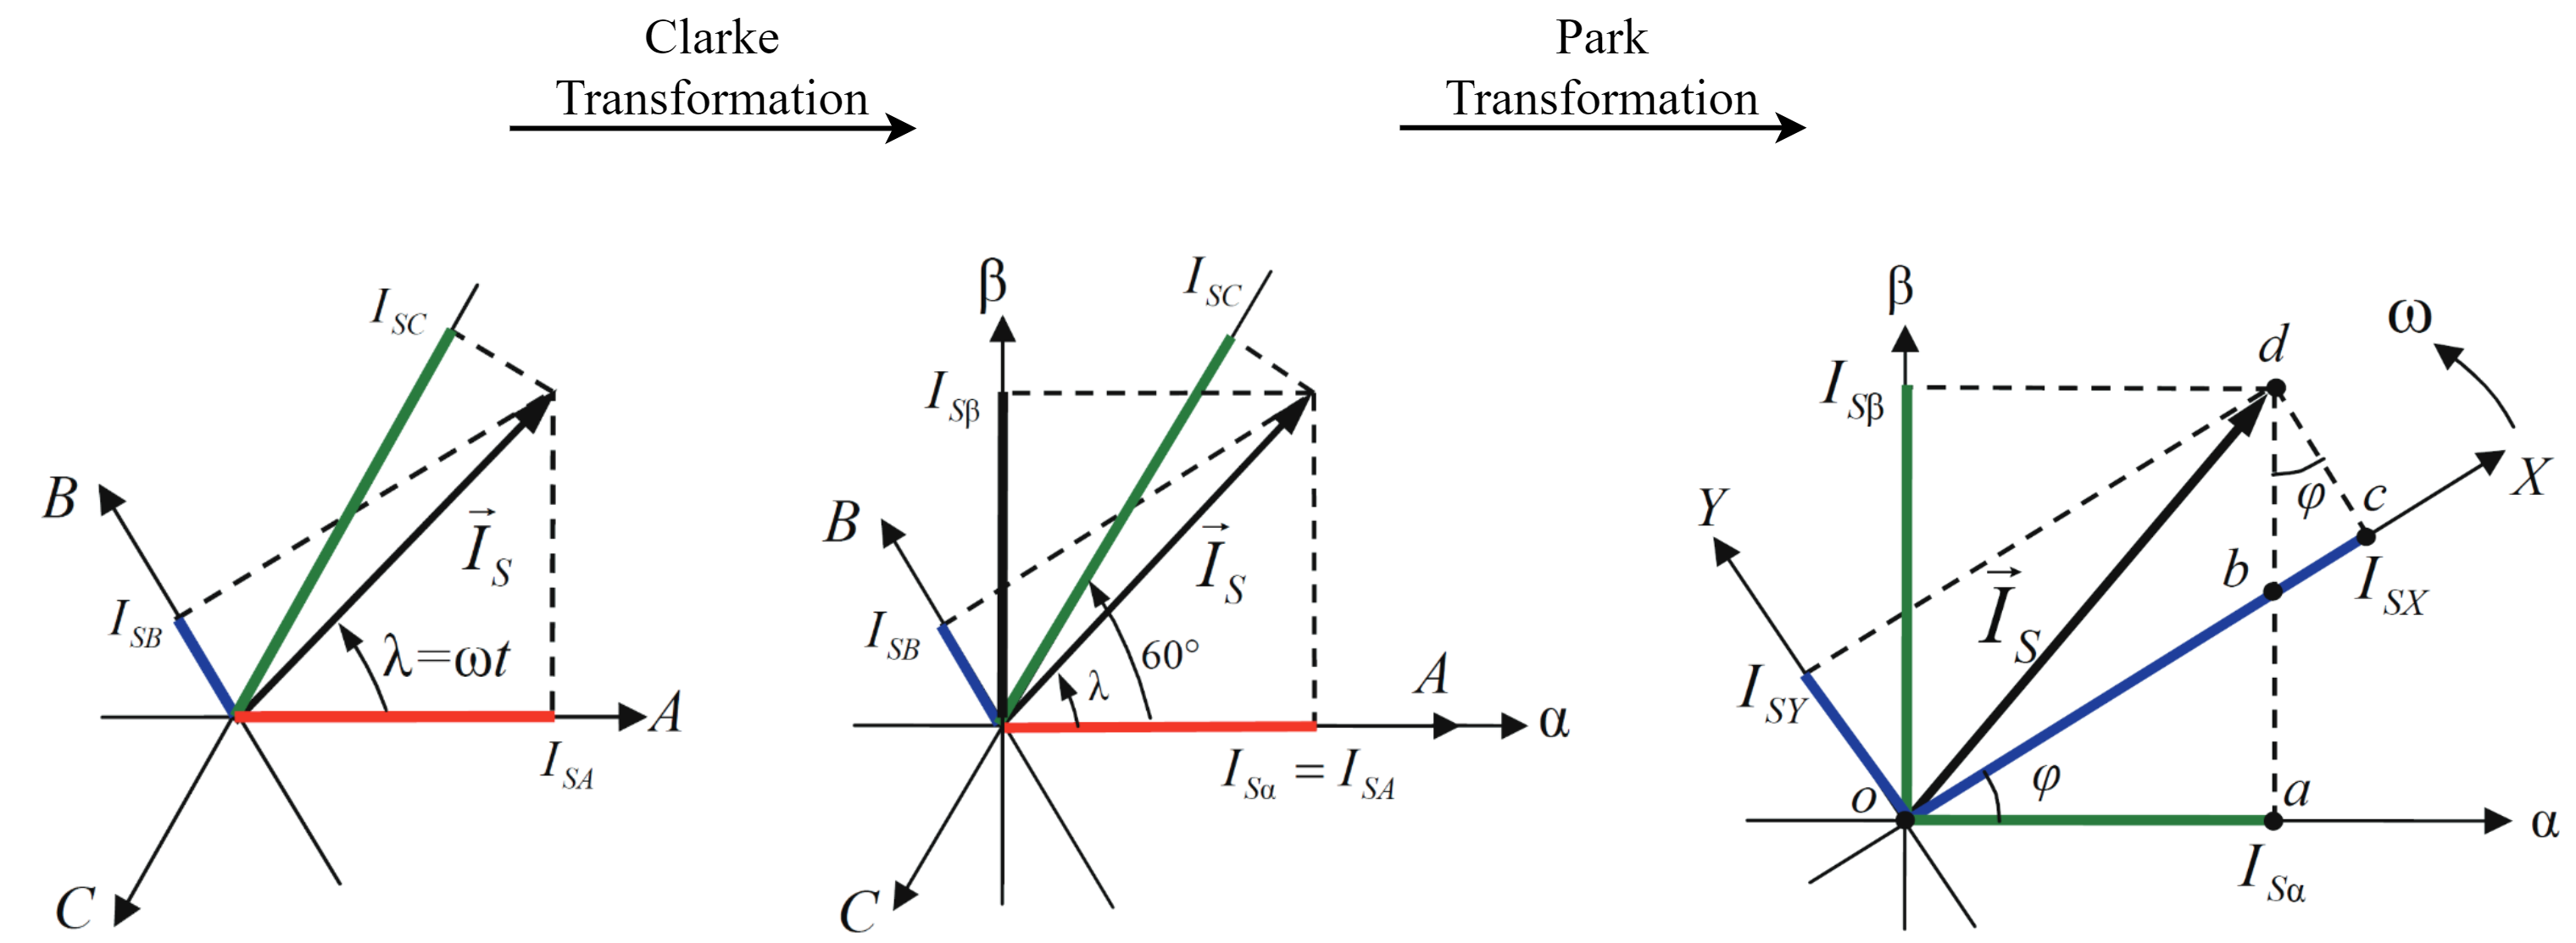
\includegraphics[width = \columnwidth]{coord_transform.png}
    \caption{Transformation of three-phase coordinate, $\alpha \beta$-coordinate, and $dq$-coordinate \autocite{Kalachev2013}.}
    \label{fig:coord_transform}
\end{figure}

Unlike the $\alpha \beta$-frame control, $dq$-frame control necessitates a synchronization method, typically provided by the phase-locked loop (PLL), which is considered a drawback of the $dq$-frame control.

\subsection{Dynamic Model of Power Controller}\label{subsec:ch3/sec2/sub2}
To observe dynamics of the power system, the real-/reactive-power controller in $dq$-frame will be analyzed.
% To observe dynamics of the power system, the simplified diagram in Figure~\cref{fig:grid_following} of a current-controlled real-/reactive-power controller in $dq$-frame will be analyzed.

% \begin{figure}[htbp]
%     \centering
%     \includegraphics[width = \columnwidth]{graphics/grid_following.png}
%     \caption{Schematic diagram of a current-controlled real-/reactive-power controller in dq-frame.}
%     \label{fig:grid_following}
% \end{figure}

The AC system voltage in the VSC system can be expressed as
\begin{equation}
    \begin{array}{l}
        V_{s a}(t)=\widehat{V}_{s} \cos \left(\omega_{0} t+\theta_{0}\right) \\
        V_{s b}(t)=\widehat{V}_{s} \cos \left(\omega_{0} t+\theta_{0}-\frac{2 \pi}{3}\right), \\
        V_{s c}(t)=\widehat{V}_{s} \cos \left(\omega_{0} t+\theta_{0}-\frac{4 \pi}{3}\right),
    \end{array}
\end{equation}
where $\widehat{V}_s$ is the peak value of the line-to-neutral voltage, $\omega_0$ is the frequency of the AC system, and $\theta_0$ is the angle of initial phase of the source. The space phasor equivalent of $V_{s-a b c}$ is
\begin{equation}
    \begin{aligned}
        \label{eq:v_phasor}
        \vec{V}_s(t)=\widehat{V}_s e^{j\left(\omega_0 t+\theta_0\right)}.
    \end{aligned}
\end{equation}

Dynamics of the AC side of the system are described by the following space-phasor equation:
\begin{equation}
    \label{eq:inv_dynamic}
    \begin{aligned}
        L \frac{d \vec{i}}{d t}=-R \vec{i}+\vec{V}_t-\vec{V}_s.
    \end{aligned}
\end{equation}

This can be decomposed into real and imaginary components:
\begin{equation}
    \label{eq:inv_nonlinear}
    \begin{aligned}
        & L \frac{d i_d}{d t}=L \omega(t) i_q-R i_d+V_{t d}-\widehat{V}_s \cos \left(\omega_0 t+\theta_0-\rho\right), \\
        & L \frac{d i_q}{d t}=-L \omega(t) i_d-R i_q+V_{t q}-\widehat{V}_s \sin \left(\omega_0 t+\theta_0-\rho\right), \\
        & \frac{d \rho}{d t}=\omega(t).
    \end{aligned}
\end{equation}

The further investigation will lead to:
\begin{equation}
    \begin{aligned}
        & L \frac{d i_d}{d t}=L \omega_0 i_q-R i_d+V_{t d}-\widehat{V}_s, \\
        & L \frac{d i_q}{d t}=-L \omega_0 i_d-R i_q+V_{t q}.
    \end{aligned}
\end{equation}
which describe a second-order linear system influenced by the steady input $\widehat{V}_s$. Therefore, with $V_{t d}$ and $V_{t q}$ as DC values, $i_d$ and $i_q$ also remain DC in the steady state. The method that ensures $\rho(t)=\omega_0 t+\theta_0$ is the PLL \autocite{book_yazdani_2010}. The next section outlines the PLL's structure, modeling, and stabilization.

\subsection{Grid Synchronization}\label{subsec:ch3/sec2/sub3}
PLL ensures the $dq$ frame aligns with the grid voltage phasor's rotation \autocite{cole2010vsc, 5637778}. Figure~\cref{fig:pll_basic} illustrates the fundamental-frequency model of a PLL. 

\begin{figure}[htbp]
    \centering
    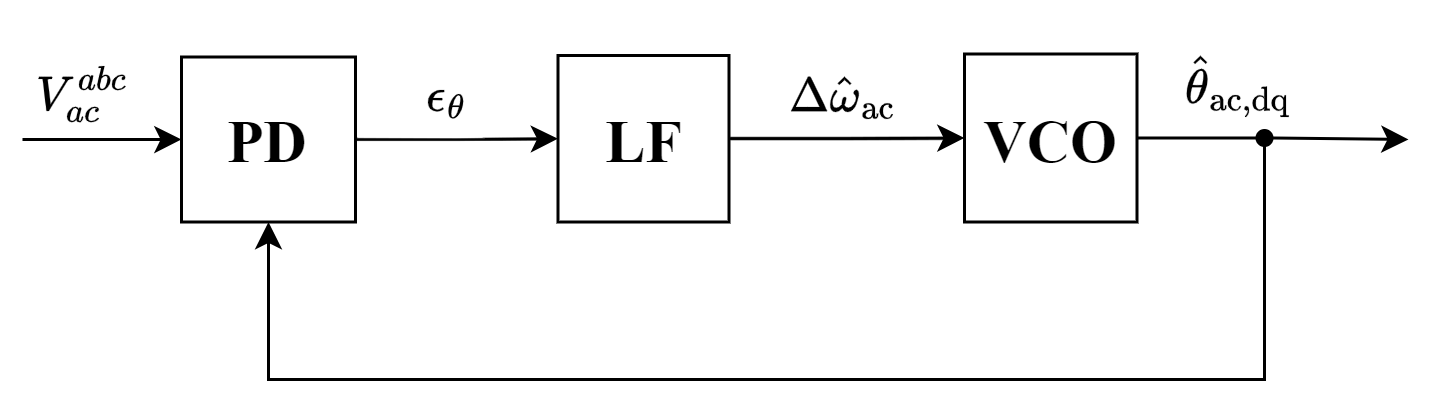
\includegraphics[width = 0.8\columnwidth]{pll_basic.png}
    \caption{Basic scheme of a PLL \autocite{Milano_2019_ess}.}
    \label{fig:pll_basic}
\end{figure}
Key components include \autocite{Milano_2019_ess}:
\begin{itemize}
    \item The Phase Detector (PD) evaluates the three-phase voltage vector, $V_{ac}^{abc}$, at the connection bus and computes the phase angle offset, $\epsilon_\theta$, between the measured phase angle, $\hat{\theta}_\mathrm{ac}$, and the $dq$ frame angle estimated by the PLL, $\hat{\theta}_{\mathrm{ac}, \mathrm{dq}}$. The voltage first transitions from ‘$abc$’ to ‘$\alpha\beta\gamma$’, and subsequently to ‘$dqo$’ components.
     \item The Loop Filter (LF) processes the error $\epsilon_\theta$ between actual and estimated voltage phase angles. Despite various LF configurations, they are typically designed as perfect tracking controllers that ensure $\epsilon_\theta = 0$ in steady state. Notably, the LF output estimates the frequency deviation at the connection bus, $\Delta \hat{\omega}_{\mathrm{ac}}$.
     \item The Voltage Controlled Oscillator (VCO) uses the bus frequency shift $\Delta \hat{\omega}_{\mathrm{ac}}$ to estimate the $dq$-frame phase angle $\hat{\theta}_{\mathrm{ac}, \mathrm{dq}}$, generally operating with an integrator that stabilizes to $\Delta \hat{\omega}_{\mathrm{ac}}$.
\end{itemize}

More detailed control diagram is presented in Figure~\cref{fig:pll_control}, forming a dynamic equation: 
\begin{equation}
     \frac{d\rho}{dt} = \hat{V}_{s} H(p) (\omega_{0} t + \theta_{0} - \rho),
\end{equation}
\noindent which represents a feedback control loop in which $\omega_{0} t + \theta_{0}$ is the reference input, $\rho$ is obtained angle, and $H(s)$ is the compensator transfer function. The dynamic performance of the PLL is greatly affected by the compensator H(s). In real conditions, the compensator should be able to deal with unbalanced and/or harmonically distorted three-phase voltages. In this work, we assume the ideal balanced voltage conditions and apply PLL compensator as PI controller only.

\begin{figure}[htbp]
    \centering
    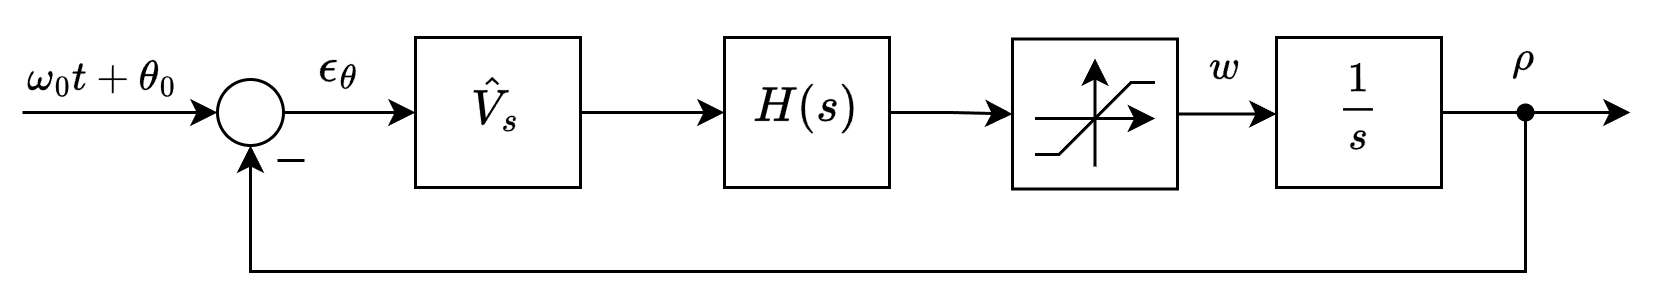
\includegraphics[width = \columnwidth]{pll_control.png}
    \caption{Basic inverter control block diagram of PLL \autocite{6739414}}
    \label{fig:pll_control}
\end{figure}

\subsection{Control}\label{subsec:ch3/sec2/sub4}
Suggesting ideal angle matching within PLL and applying Park transformation the expression of the terminal voltage of the AC side of the converter, $V_{t}^{abc}$, can be written in the $dq$ frame as follows:
\begin{equation}
    v_{\mathrm{t}, \mathrm{dq}}(t)=\left[\begin{array}{c}
v_{\mathrm{t}, \mathrm{~d}}(t) \\
v_{\mathrm{t}, \mathrm{q}}(t)
\end{array}\right]=\mathbf{P} \frac{v_{\mathrm{dc}}}{2}\left[\begin{array}{c}
m_{\mathrm{a}}(t) \\
m_{\mathrm{b}}(t) \\
m_{\mathrm{c}}(t)
\end{array}\right]=\frac{v_{\mathrm{dc}}}{2}\left[\begin{array}{c}
m_{\mathrm{d}}(t) \\
m_{\mathrm{q}}(t)
\end{array}\right],
\label{eq:v_dq_transf}
\end{equation}
where $\mathbf{P}$ is the Park tensor, the system under balanced conditions and the nominal frequency.

The expression of the complex power of the AC side of the VSC, $\bar{s}_{\mathrm{ac}}$, projected onto the $dq$ frame is:
\begin{equation}
    \begin{aligned}
        \bar{s}_{\text{ac}}(t) &= p_{\text{ac}}(t) + j q_{\text{ac}}(t) = \frac{3}{2} \left( \bar{v}_{\text{ac,dq}}(t) \bar{i}_{\text{ac,dq}}^*(t) \right) \\
        &= \frac{3}{2} \left[ v_{\text{ac,d}}(t) i_{\text{ac,d}}(t) + v_{\text{ac,q}}(t) i_{\text{ac,q}}(t) \right. \\
        &\quad \left. +\, j \left( v_{\text{ac,q}}(t) i_{\text{ac,d}}(t) - v_{\text{ac,d}}(t) i_{\text{ac,q}}(t) \right) \right],
    \end{aligned}
\end{equation}

Thus:
\begin{equation}
    \begin{aligned}
        \begin{array}{l}
            p_{\mathrm{ac}}(t)=\operatorname{Re}\left\{\bar{s}_{\mathrm{ac}}(t)\right\}=\displaystyle\frac{3}{2}\left(v_{\mathrm{ac}, \mathrm{~d}}(t) i_{\mathrm{ac}, \mathrm{~d}}(t)+v_{\mathrm{ac}, \mathrm{q}}(t) i_{\mathrm{ac}, \mathrm{q}}(t)\right) \\[1em]
            q_{\mathrm{ac}}(t)=\operatorname{Im}\left\{\bar{s}_{\mathrm{ac}}(t)\right\}=\displaystyle\frac{3}{2}\left(v_{\mathrm{ac}, \mathrm{q}}(t) i_{\mathrm{ac}, \mathrm{~d}}(t)-v_{\mathrm{ac}, \mathrm{~d}}(t) i_{\mathrm{ac}, \mathrm{q}}(t)\right) .
        \end{array}
    \end{aligned}
\end{equation}
where $v_{ac,d}$ and $v_{ac,q}$ are the $dq$-frame voltage components of the AC system and cannot be controlled by the VSC system. If the PLL is in a steady state, $v_{ac,q}=0$ and can be rewritten as

\begin{equation}
    \begin{aligned}
        \begin{array}{l}
            p_{\mathrm{ac}}(t) = \displaystyle\frac{3}{2} v_{\mathrm{ac}, \mathrm{~d}}(t)i_{\mathrm{ac}, \mathrm{~d}}(t), \\[1em]
            q_{\mathrm{ac}}(t) = -\displaystyle\frac{3}{2} V_{sd}(t)i_q(t).
        \end{array}
    \end{aligned}
\end{equation}

Based on that, $p_{\mathrm{ac}}(t)$ and $q_{\mathrm{ac}}(t)$ can be controlled by $id$ and $iq$, respectively.

\begin{equation}
    \begin{aligned}
        i_{dref}(t) & =\frac{2}{3V_{sd}} P_{sref}(t) \\[1em]
        i_{qref}(t) & =-\frac{2}{3 V_{sd}} Q_{sref}(t)
    \end{aligned}
\end{equation}

\textbf{Grid-Following Mode}. In most cases, where an inverter is involved in delivering power from DER or ESS to the grid, it works in grid following mode, where real (DC) and reactive (AC) powers (voltages) are regulated by means of the components of the current $i_{ac}^{abc}$ \autocite{720325}. 
The control scheme consists of current control loop and reference signal generator. It allows us to protect the VSC against possible overcurrents. Moreover, current-mode control includes dynamic performance, overload rejection, and robustness against changes in load parameters.

The scheme of the inner current control loop of the VSC coupled to the converter is shown in Figure~\cref{fig:inv_cc}.

\begin{figure}[htbp]
    \centering
    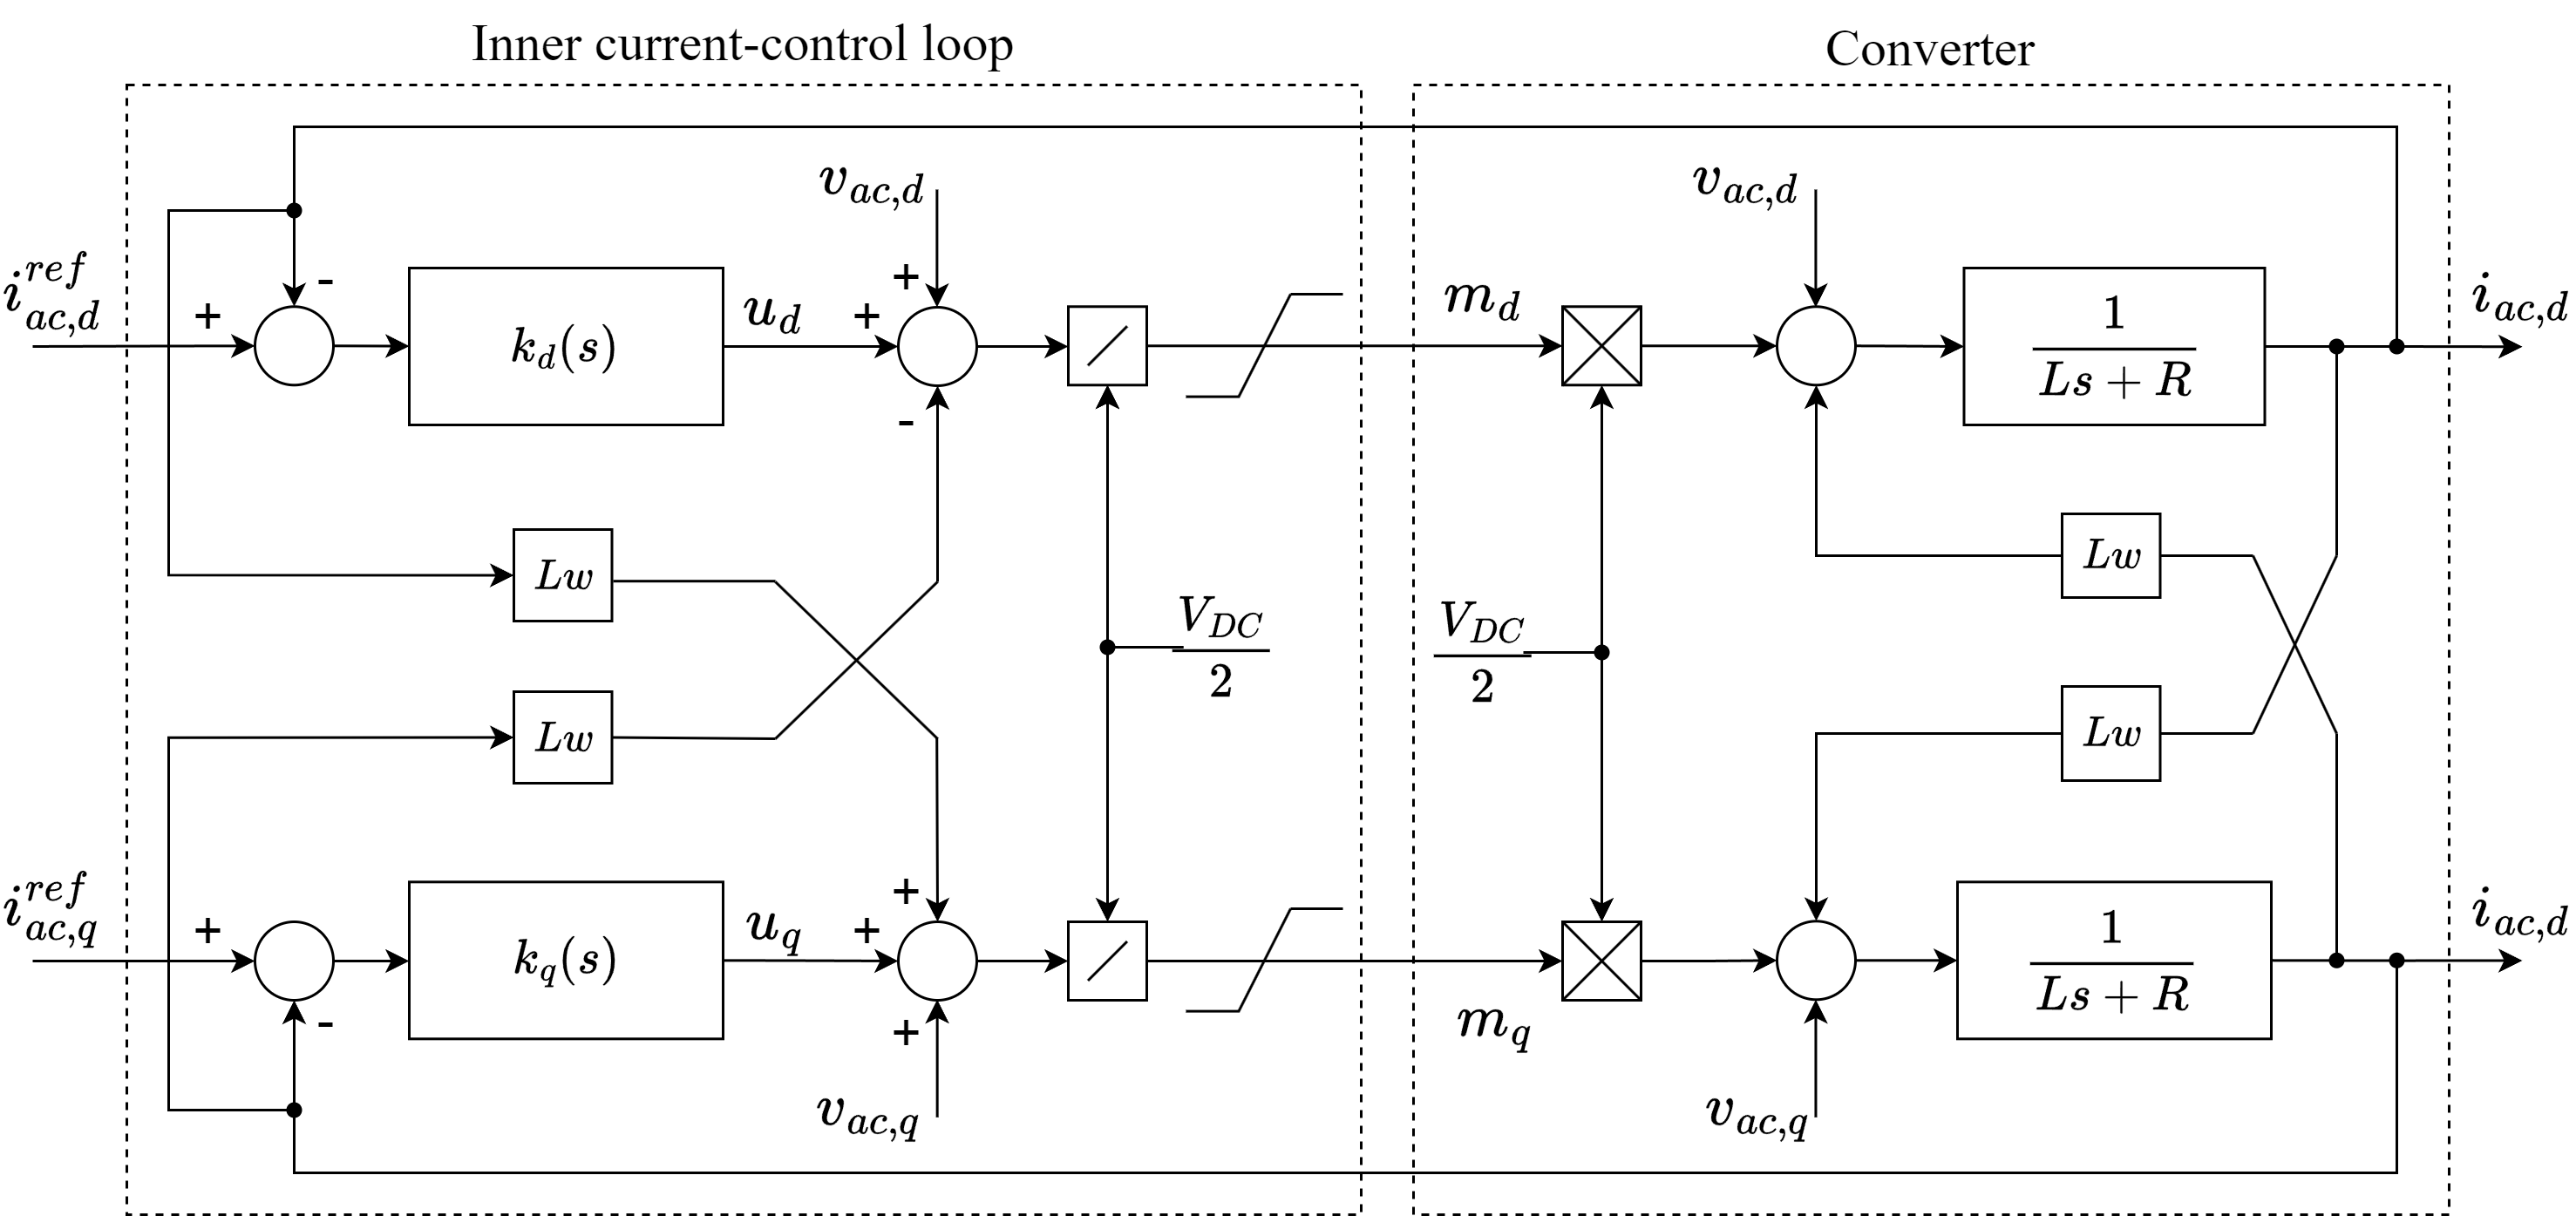
\includegraphics[width = 1\columnwidth]{inv_cc.png}
    \caption{VSC grid-following control diagram in the dq frame}
    \label{fig:inv_diagram_gfl}
\end{figure}

The $dq$-frame control of the active/reactive-current controller here is based on \ref{eq:inv_nonlinear}. Assuming a steady-state and setting $\omega(t)$ to $\omega_0$, we conclude
\begin{equation}
    \begin{array}{l}
L \displaystyle\frac{d i_{d}}{d t}=L \omega_{0} i_{q}-R i_{d}+V_{t d}-V_{s d} \\[1em]
L \displaystyle\frac{d i_{q}}{d t}=-L \omega_{0} i_{d}-R i_{q}+V_{t q}-V_{s q}
\end{array}
\end{equation}

As can be seen, $L\omega_0$ terms bring coupling to the $id$ and $iq$ dynamics. Applying $dq$ transformation \ref{eq:v_dq_transf} we can determine $m_d$ and $m_q$ to decouple the dynamics as 
\begin{equation}
    \begin{aligned}
m_{d} & =\frac{2}{V_{D C}}\left(u_{d}-L \omega_{0} i_{q}+V_{s d}\right) \\
m_{q} & =\frac{2}{V_{D C}}\left(u_{q}+L \omega_{0} i_{d}+V_{s q}\right)
\end{aligned}
\end{equation}
where $u_d$ and $u_q$ are two control inputs, which are the outputs of two corresponding compensators, shown in Figure~\cref{fig:inv_cc_pi}. Basically, $k_d(s)$ can be a simple proportional-integral (PI) compensator to track the DC reference signal.

\begin{figure}[htbp]
    \centering
    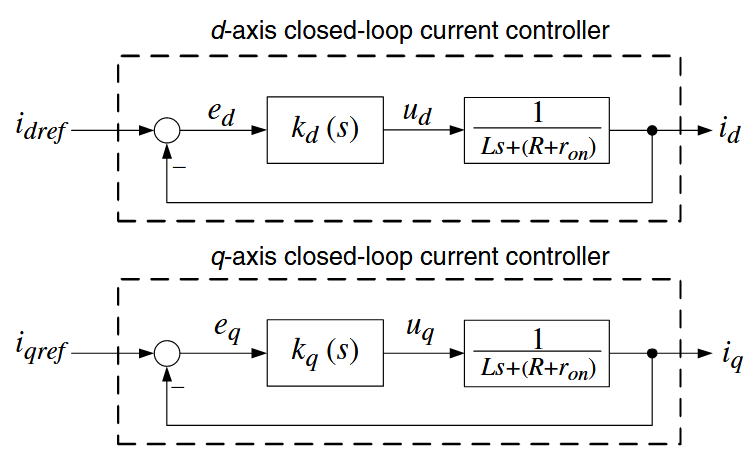
\includegraphics[width = 0.7\columnwidth]{inv_cc_pi.png}
    \caption{Simplified block diagram of the current-controlled VSC \autocite{book_yazdani_2010}.}
    \label{fig:inv_cc_pi}
\end{figure}

Let us assume PI regulator
\begin{equation}
    k_{d}(s)=\frac{k_{p} s+k_{i}}{s},
\end{equation}
where $k_p$ denotes the proportional gain and $k_i$ represents the integral gain. 

It can be seen from Figure~\cref{fig:inv_cc_pi}, that the transfer function of the closed-loop system can be reduced to first order
\begin{equation}
    \frac{I_{d}(s)}{I_{d r e f}(s)}=G_{i}(s)=\frac{1}{\tau_{i} s+1},
\end{equation}
in case of
\begin{equation}
    \begin{array}{l}
k_{p}=L / \tau_{i}, \\
k_{i}=\left(R+r_{o n}\right) / \tau_{i}.
\end{array}
\label{eq:cc_pi}
\end{equation}
where $\tau_i$ is the time constant of the resultant closed-loop system. The final view of the averaged model of inverter with control blocks in grid-following mode will take the form:
\begin{figure}[htbp]
    \centering
    \includegraphics[width = 1\columnwidth]{grid_following.png}
    \caption{Simplified block diagram of the VSC in grid-following mode}
    \label{fig:inv_cc}
\end{figure}

\textbf{Grid-Forming Mode}. In case of system transit to island mode without an external grid, an inverter switches to grid-forming mode. In this mode, the goal is to maintain the load voltage's amplitude and frequency despite fluctuations in load current. To prevent switching current harmonics penetrate into the load, $C_f$ appears to $RL$ filter. The control here can be realized here in $dq$-frame as in grid-following mode, while the angle for transformations, $\rho$, is obtained from the output of a VCO whose input is $d\rho/dt = \omega(t)$. $\omega(t)$ can be set as nominal frequency of the power system, $\omega_0$, or it can be dynamically controlled in a variable-frequency environment \autocite{5275592}. The averaged model of inverter with control blocks in grid-forming mode has the form:
\begin{figure}[htbp]
    \centering
    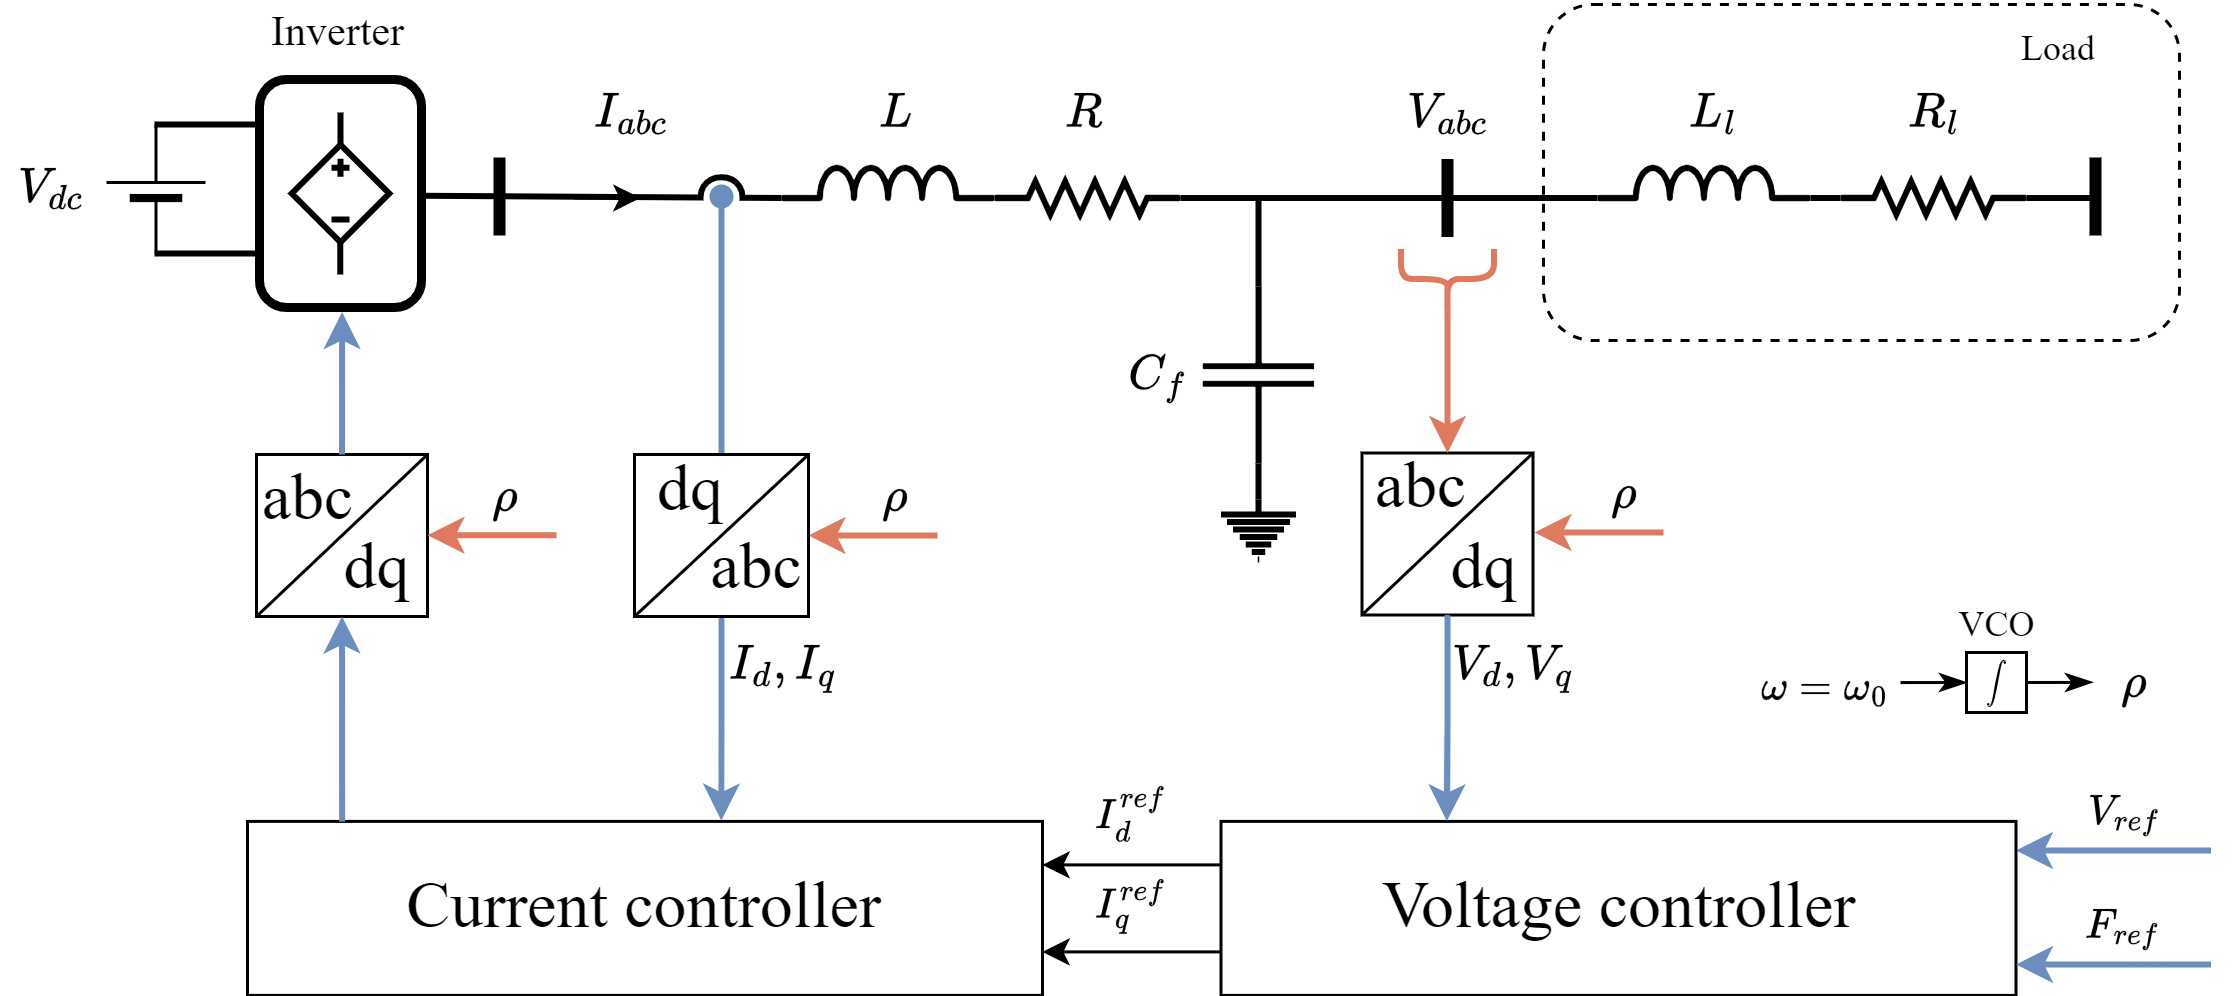
\includegraphics[width = 0.95\columnwidth]{grid_forming.png}
    \caption{Simplified block diagram of the VSC in grid-forming mode}
    \label{fig:inv_gf}
\end{figure}

The voltage, delivered to the load in this case will take the form in terms of its $dq$-frame components:
\begin{equation}
    \begin{aligned}
        C_{f} \frac{d V_{s d}}{d t} & =C_{f}\left(\omega V_{s q}\right)+i_{d}-i_{L d} \\
        C_{f} \frac{d V_{s q}}{d t} & =-C_{f}\left(\omega V_{s d}\right)+i_{q}-i_{L q},
    \end{aligned}
    \label{eq:inv_vc}
\end{equation}
where $d\rho/dt$ has been replaced by $\omega(t)$. 

Equations \ref{eq:inv_vc} illustrate the dynamics of $V_{sd}$ and $V_{sq}$. Here, $V_{sd}$ and $V_{sq}$ represent system outputs, while $i_d$, $i_q$, and $\omega$ act as control inputs. Furthermore, $i_d$ and $i_q$ respond to the d- and q-axis current controllers of the VSC system, based on $i_{dref}$ and $i_{qref}$, respectively.

As shown in Figure~\cref{fig:inv_vc}, $V_{sd}$ and $V_{sq}$ can be controlled by $i_{dref}$ and $i_{qref}$, while also being interconnected, reflecting the effects of $i_{Ld}$ and $i_{Lq}$. This relation is determined as follows
\begin{equation}
    \begin{array}{l}
        i_{d r e f}=u_{d}-C_{f}\left(\omega V_{s q}\right)+i_{L d}, \\
        i_{q r e f}=u_{q}+C_{f}\left(\omega V_{s d}\right)+i_{L q} .
    \end{array}
\end{equation}
where $u_d$ and $u_q$ are two new control inputs, which are the outputs of two independent compensators. It can be seen that decoupling feed-forward compensation are required, which is similar to the one utilized to decouple $i_d$ and $i_q$ in a current-controlled VSC. The final view of the control diagram in the $dq$ frame is shown in Figure~\cref{fig:inv_diagram_gfm}.

\begin{figure}[htbp]
    \centering
    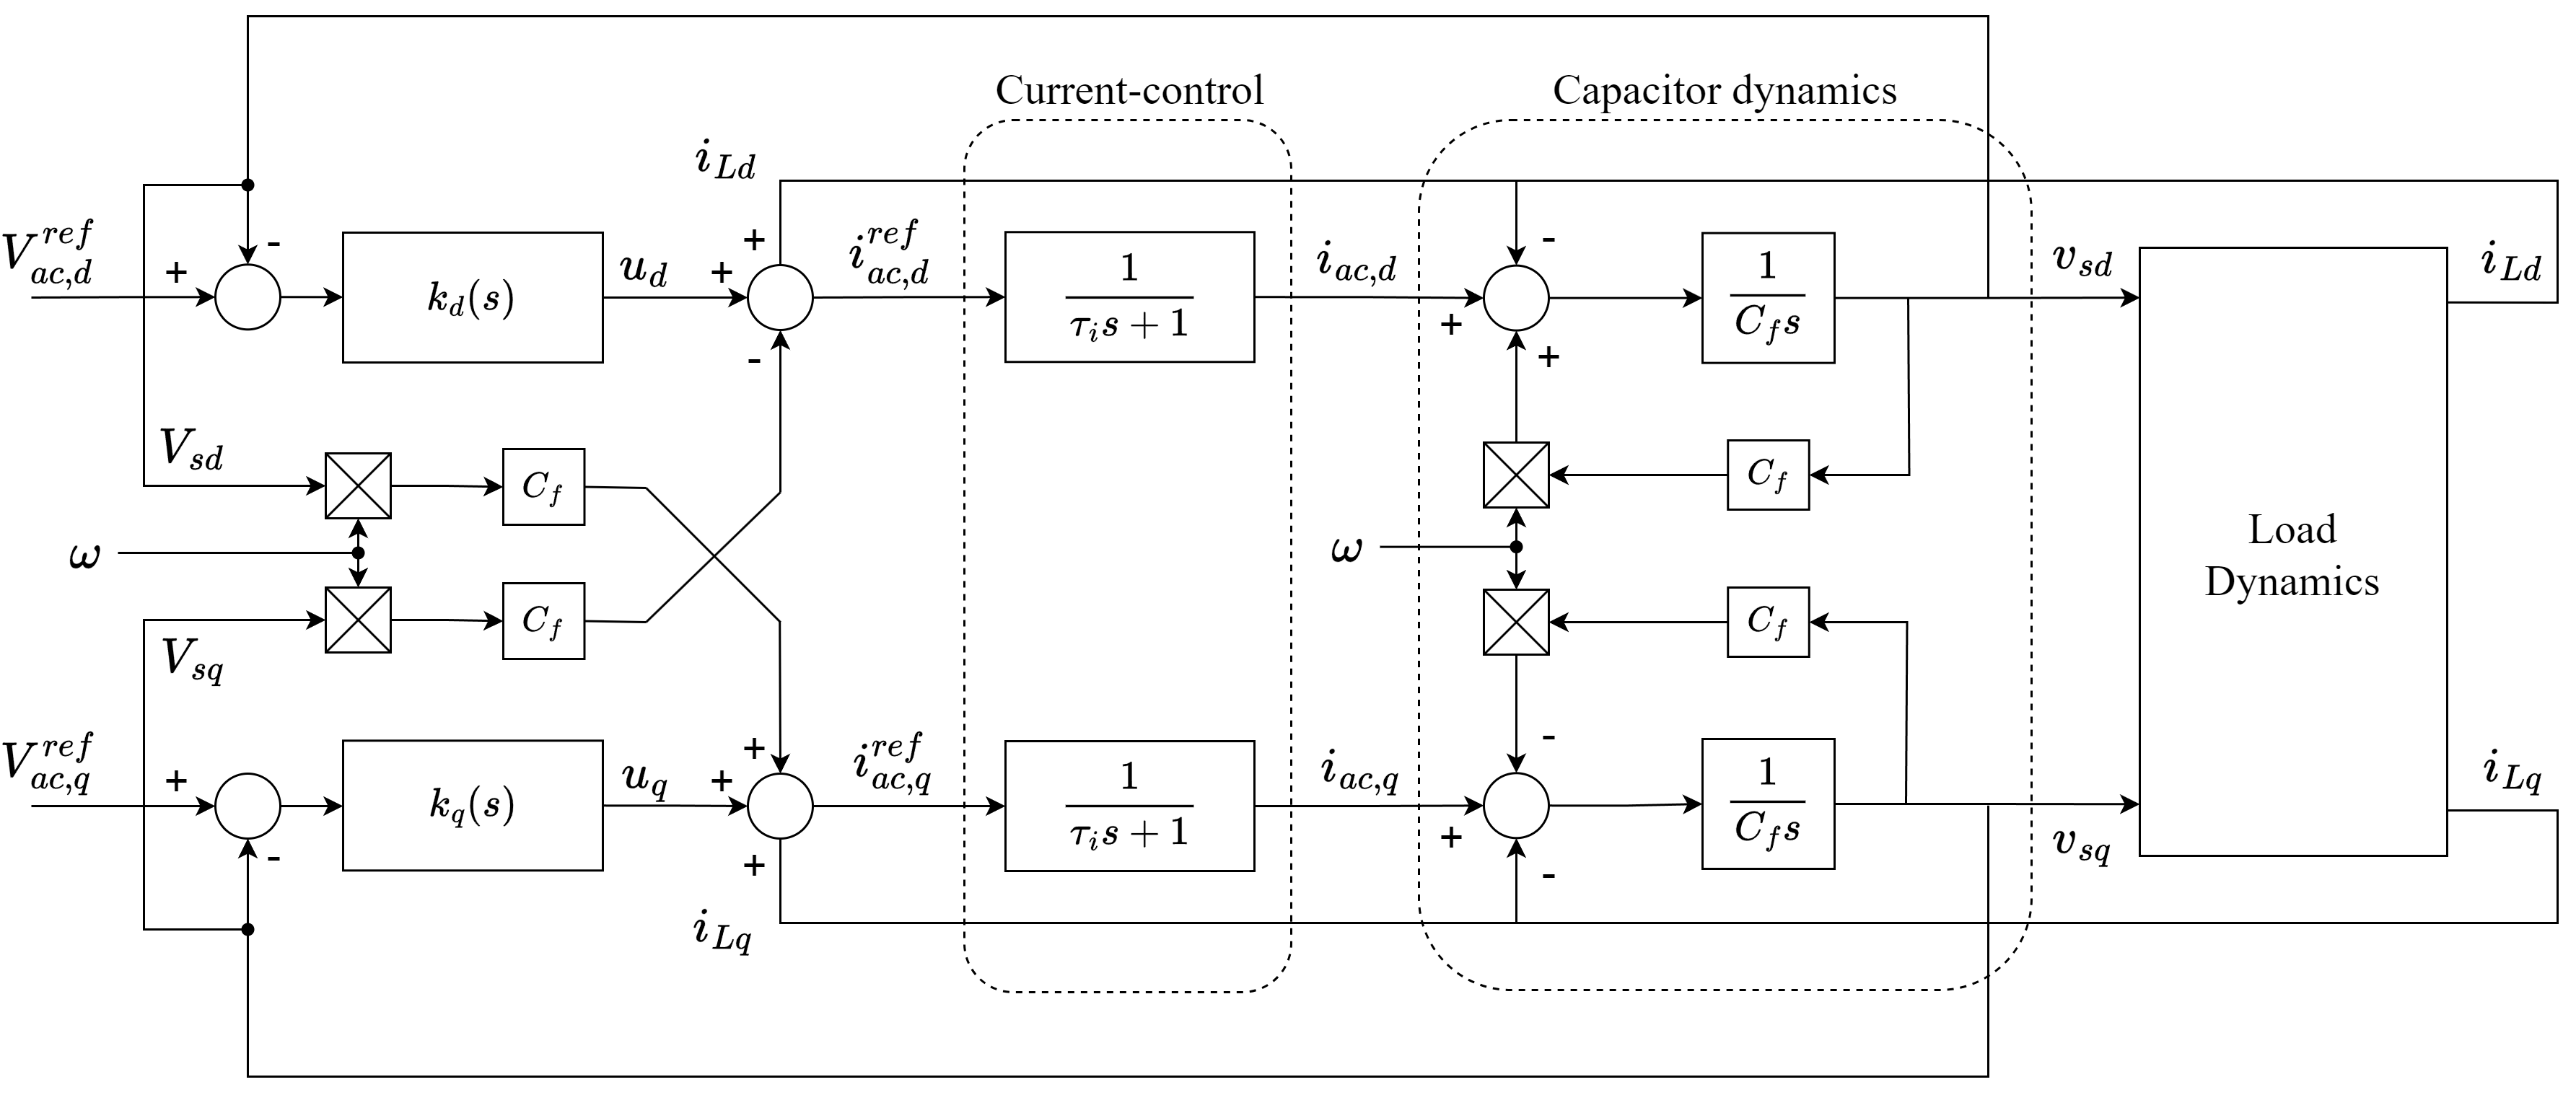
\includegraphics[width = 1\columnwidth]{inv_vc2.png}
    \caption{VSC grid-forming control diagram in the dq frame}
    \label{fig:inv_diagram_gfm}
\end{figure}

The first compensator can be processed as $e_d = V_{sdref}-V_{sd}$ and generates $u_d$. The other compensator processes $e_q = V_{sqref}-V_{sq}$ and generates $u_q$. Then $i_{dref}$ and $i_{qref}$ go to the corresponding current control loops on the $d$- and $q$ axes. The control diagram can be simplified to that of Figure~\cref{fig:inv_vc}.

\begin{figure}[htbp]
    \centering
    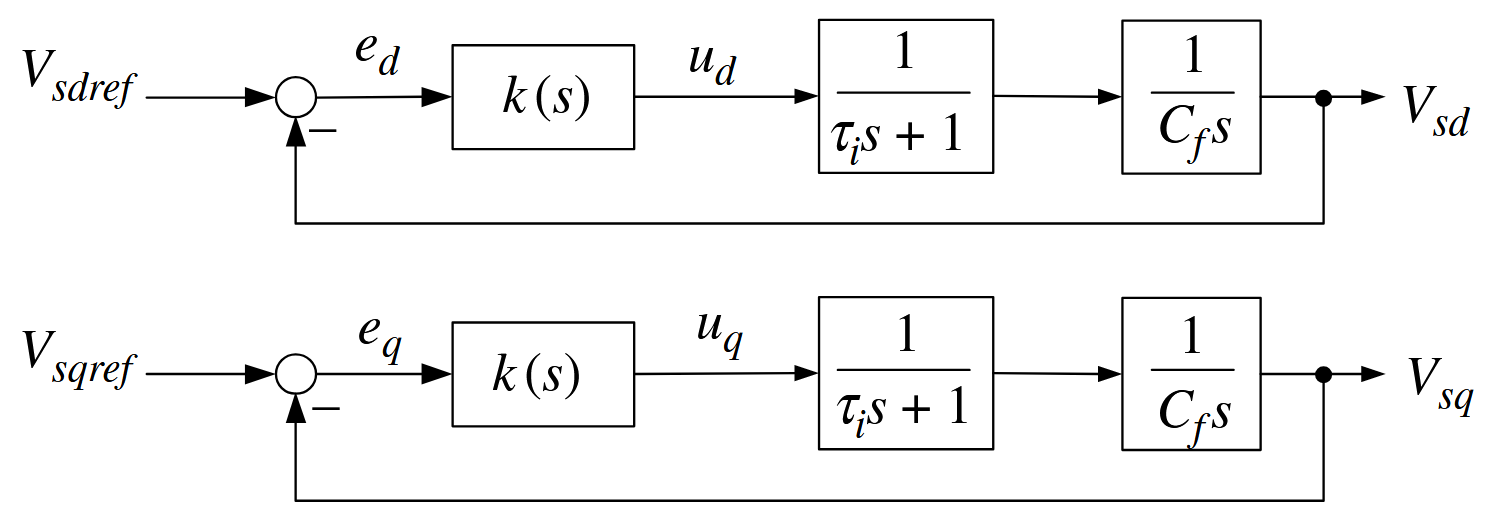
\includegraphics[width = 0.8\columnwidth]{inv_vc_pi.png}
    \caption{Simplified grid-forming control block diagram in the dq frame \autocite{book_yazdani_2010}}
    \label{fig:inv_vc}
\end{figure}

% \subsection{Parameters estimation}

\section{Transmission Lines}\label{sec:ch3/sec3}
Transmission lines (TL) are long conductors, suspended at a safe distance from the ground, in which the conductive wires are isolated from each other and from the external environment and protected by insulation and armor through which electrical energy is transmitted. TLs are characterized by a significant feature; they are elements with distributed length parameters. Accurate calculation of topologies containing such elements leads to complex calculations, so in practical calculations, power lines are often considered as elements with concentrated parameters. This assumption is valid for overhead lines up to 300-350 km and for underground cable lines up to 50-70 km \autocite{Gerasimenko2008}. The length of distributed electrical networks is significantly shorter, and they are often classified as local electrical networks, which can be considered objects with concentrated parameters in all cases \autocite{borovikov1977electric}. Thus, it can be assumed with sufficient accuracy that series resistance and series reactance are concentrated in the middle of the line, and conductance and susceptance are at the ends. These parameters can be deduced from the per-unit length resistance $R_L$, inductance $L_L$ and capacitance $C_L$ of the line \autocite{LIU2023109321}. So-called $\pi$-branch model can be used, which is represented in Figure~\cref{fig:pi_branch}. 

\begin{figure}[htbp]
    \centering
    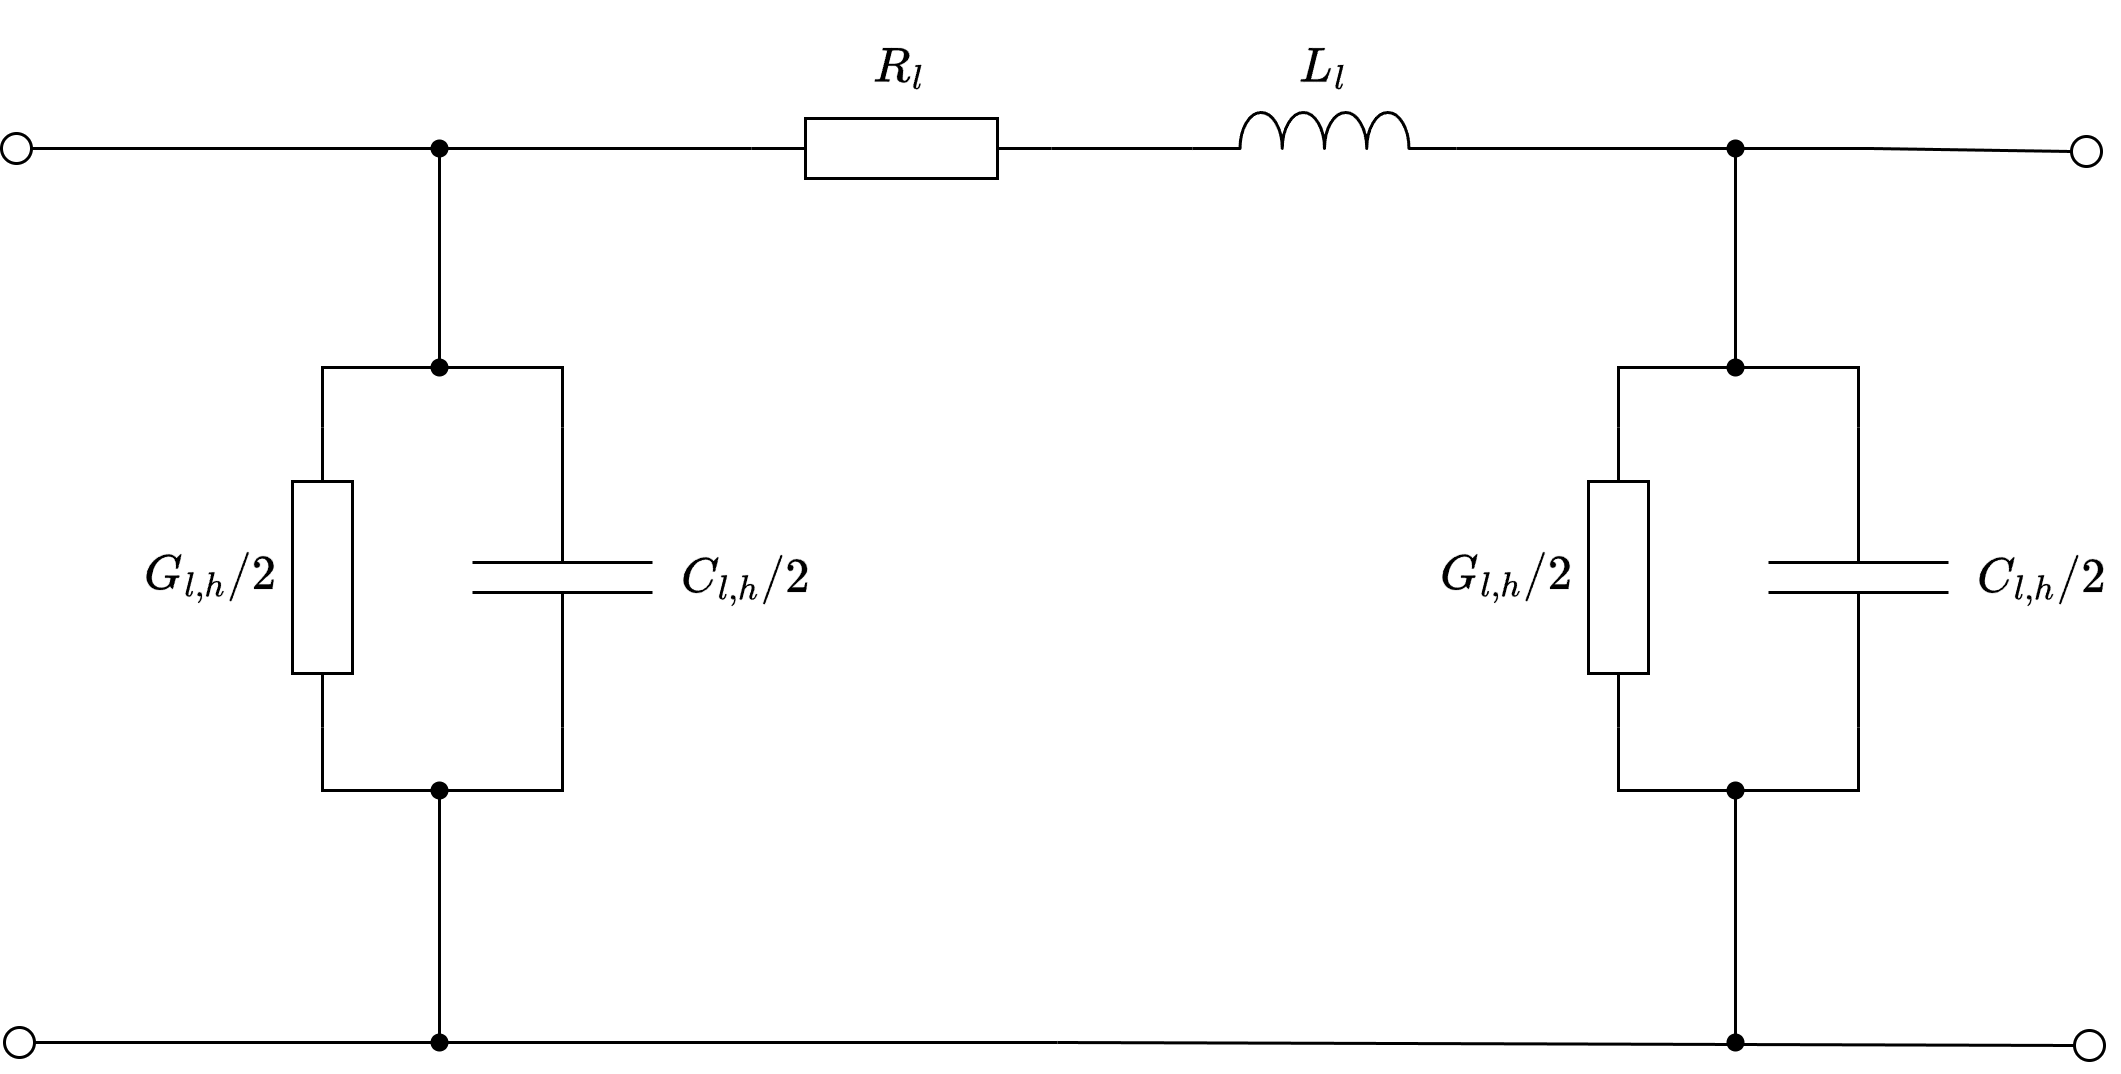
\includegraphics[width = 0.8\columnwidth]{PI-line.png}
    \caption{Line equivalent $\pi$-model with concentrated parameters}
    \label{fig:pi_branch}
\end{figure}

In the calculations of distribution electrical networks with a voltage of 0.38 to 35 kV, the replacement schemes shown in Figure~\cref{fig:pi_branch} are often simplified (the active and capacitive conductivities are not taken into account), and the scheme shown in Figure~\cref{fig:tl_04} is used. However, it should be noted that the use of simplified schemes, even in 10 to 35 kV networks, should be justified. For example, when modeling a single-phase ground fault in networks with an isolated or compensated neutral, it is not acceptable to neglect capacitive conductance. In this case, it is necessary to use the equivalent circuit shown in Figure~\cref{fig:tl_10}.

\subsection{Time domain scalar form single-section $\pi$-model with constant parameters}\label{subsec:ch3/sec3/sub1}
The model represent a single-section of $\pi$-model as shown in Figure~\cref{fig:tl_10}. 
\begin{figure}[htbp]
    \centering
    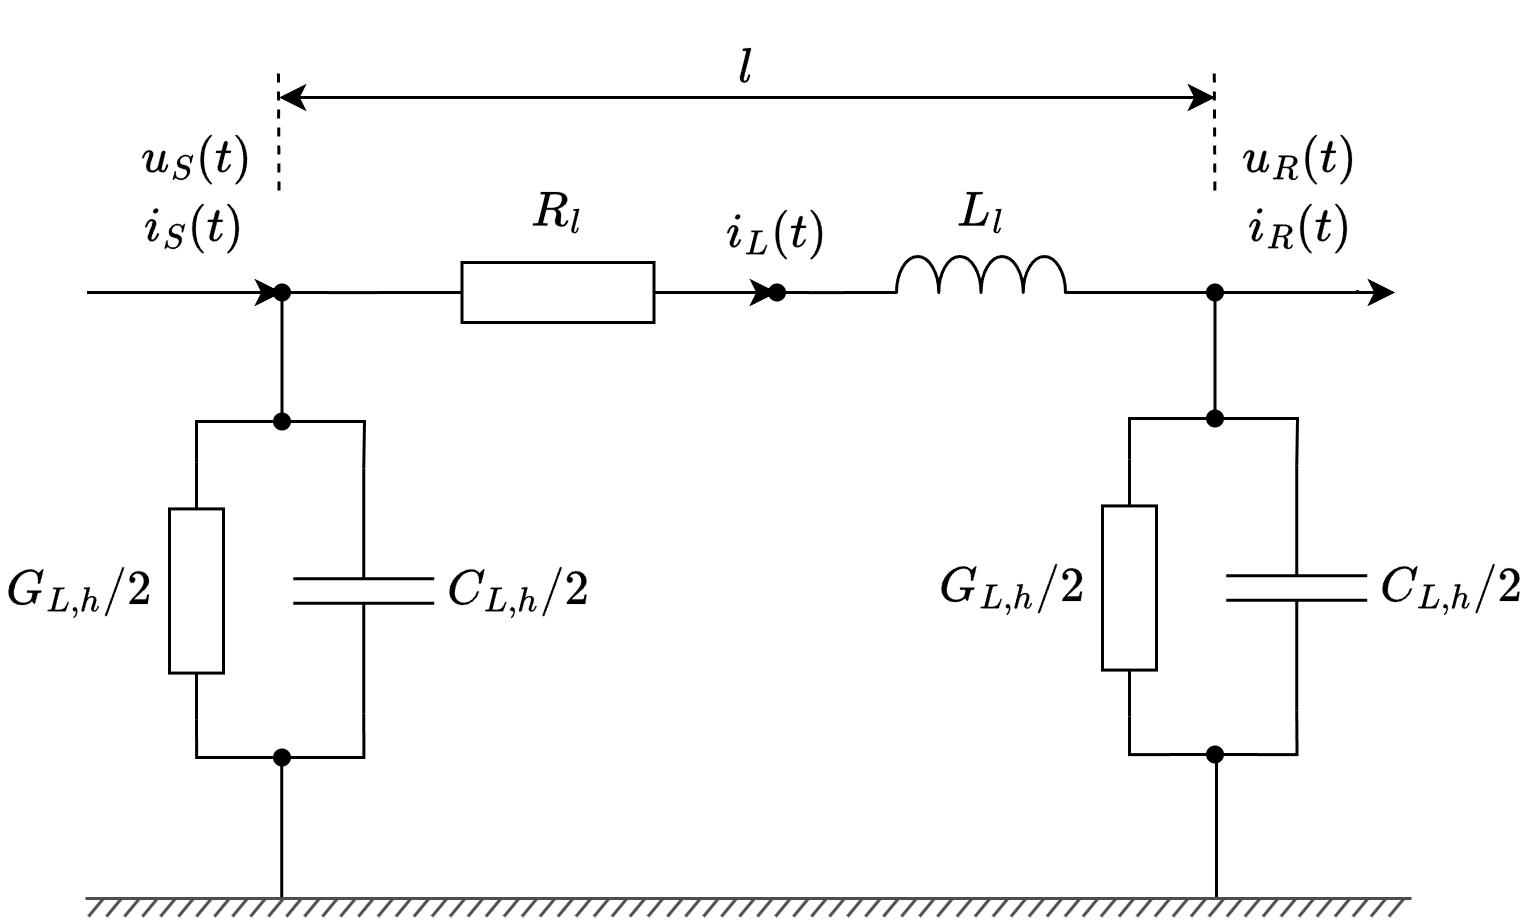
\includegraphics[width = 0.8\columnwidth]{TL_10.png}
    \caption{Equivalent circuit, time domain form single-section $\pi$ model with constant parameters}
    \label{fig:tl_10}
\end{figure}

The physical laws of this model can be described as \autocite{Liu2017TL, 9154583},
\begin{equation}
    \left\{\begin{array}{c}
        \displaystyle \mathbf{i}_{R}(t)=-\frac{\mathbf{G} l}{2} \mathbf{u}_{R}(t)-\frac{\mathbf{C} l}{2} \frac{d \mathbf{u}_{R}(t)}{d t}+\mathbf{i}_{L}(t) \\[1em]
        \displaystyle \mathbf{i}_{S}(t)=\frac{\mathbf{G} l}{2} \mathbf{u}_{S}(t)+\frac{\mathbf{C} l}{2} \frac{d \mathbf{u}_{S}(t)}{d t}+\mathbf{i}_{L}(t) \\[1em]
        \displaystyle \mathbf{0}=-\mathbf{u}_{S}(t)+\mathbf{u}_{R}(t)+\mathbf{R} l \mathbf{i}_{L}(t)+\mathbf{L} l \frac{d \mathbf{i}_{L}(t)}{d t}
    \end{array}\right.
\end{equation}
where the transmission line has a length of l. The terminal current and voltage vectors at the sending and receiving end are $i_S(t)$, $i_R(t)$, $u_S(t)$, and $u_R(t)$, respectively. Per unit length matrices for series resistance, inductance, shunt conductance, and capacitance are given by $R(x,t)$, $L(x,t)$, $G(x,t)$, and $C(x,t)$, respectively.

\subsection{Time domain scalar form RL model with constant parameters}\label{subsec:ch3/sec3/sub2}
Neglecting the shunt capacitance and conductance for a low voltage cases, an RL model is established as shown in Figure~\cref{fig:tl_04}. 
\begin{figure}[htbp]
    \centering
    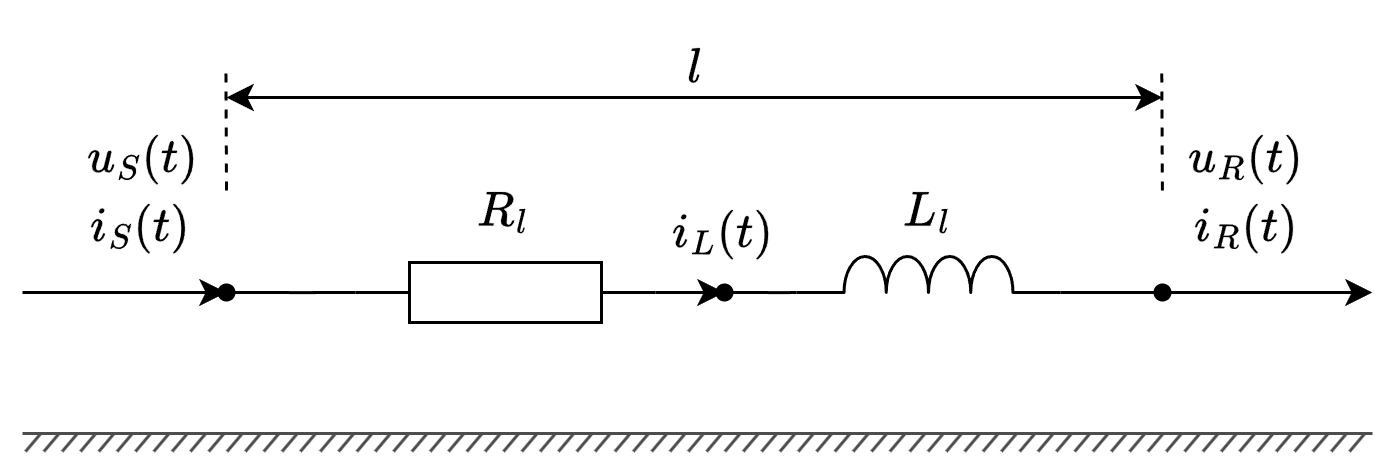
\includegraphics[width = 0.7\columnwidth]{TL_04.png}
    \caption{Equivalent circuit, time domain form RL model with constant parameters.}
    \label{fig:tl_04}
\end{figure}

The physical laws of this model can be described as \autocite{8811599},
\begin{equation}
    \left\{\begin{array}{c}
        \displaystyle \mathbf{i}_{R}(t)=\mathbf{i}_{L}(t), \quad \mathbf{i}_{S}(t)=\mathbf{i}_{L}(t), \\[1em]
        \displaystyle \mathbf{0}=-\mathbf{u}_{S}(t)+\mathbf{u}_{R}(t)+\mathbf{R} l \mathbf{i}_{L}(t)+\mathbf{L} l \frac{d \mathbf{i}_{L}(t)}{d t}.
    \end{array}\right.
\end{equation}

% \subsection{Parameters estimation}
% Several techniques have been described in the literature to estimate the parameters of the transmission line model from measurements. 

% \section{Power Transformer}

\section{Loads}\label{sec:ch3/sec4}
Prosumers, including storage systems and electric vehicles, can be modeled and integrated within the previously established current source framework, characterized by negative power generation. Conversely, the remaining $l$ loads are commonly modeled as voltage-dependent, with its active power $P$ and reactive power $Q$ adjusting according to changes in the positive sequence voltage \autocite{9369128}.
\begin{equation}\label{eq:pq_l}
    P_l = P_0(V/V_0)^\alpha, \quad Q_l = Q_0(V/V_0)^\beta,
\end{equation}

\noindent where $\alpha$ and $\beta$ are the coefficients for voltage in relation to active and reactive power, typically ranging from 0 to 2. When $\alpha = \beta = 0$, the load exhibits constant power characteristics; when $\alpha = \beta = 1$, the load behaves as a constant current source; and when $\alpha = \beta = 2$, the load acts as a constant impedance. The variable $V_0$ denotes the initial positive sequence voltage.

The initial operating point is defined by the active power $P_0$ and reactive power $Q_0$ at the initial voltage $V_0$. The active and reactive power, denoted by $P$ and $Q$, vary in accordance with the power reference provided by a measurement device, which is based on the positive sequence voltage $V$.

\section{Simulation engine}\label{sec:ch3/sec5}

In digital simulations carried out in the time domain, a system that operates continuously over time needs to be represented in a discrete form. Due to this transformation, it is not possible to directly derive or integrate the original continuous-time equations. Instead, the dynamic behavior of the system is approximated using suitable numerical techniques. To make this possible, the differential equations that describe continuous-time dynamics are rewritten as difference equations, which can then be solved step by step on a computer. The Electromagnetic Transients (EMT) simulation is widespread approach for generating this type of information \autocite{dommel1992emtp,4073845,osti_78239,277712,56581}, and is often used to validate steady-state power system analyses against transient simulations. Real-time EMT enhances DT's ability to model sensitive system operating conditions. 

% For example, for the case of an inductor, shown in Figure~\cref{fig:inductor},
% \begin{figure}[htbp]
%     \centering
%     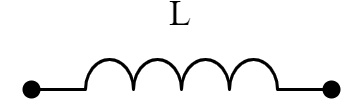
\includegraphics[width = 0.3\columnwidth]{graphics/inductor.png}
%     \caption{Inductor component}
%     \label{fig:inductor}
% \end{figure}
% the relation between the voltage across it and its current is given by
% \begin{equation}
%     V_{L}(t)=L \frac{d i_{L}(t)}{d t}
% \end{equation}

% Solving for the voltage,
% \begin{equation}
% \begin{aligned}
%     \begin{array}{c}
% \displaystyle V_{L} d t=L d i_{L}(t) \\[1em]
% \displaystyle \int_{t-\Delta t}^{t} V_{L} d t=L \int_{t-\Delta t}^{t} d i_{L}(t) \\[1em]
% \displaystyle \int_{t-\Delta t}^{t} V_{L} d t=L\left[i_{L}(t)-i_{L}(t-\Delta t)\right]
% \end{array}
% \end{aligned}
% \end{equation}
% where $\Delta t$ is the discretization time step. Approximating the left-hand side with the trapezoidal formula, we obtain
% \begin{equation}
%     \frac{V_{L}(t)+V_{L}(t-\Delta t)}{2} \Delta t=L\left[i_{L}(t)-i_{L}(t-\Delta t)\right]
% \end{equation}

% Then the voltage across the inductor is
% \begin{equation}
%     V_{L}(t)=\frac{2 L}{\Delta t} i_{L}(t)+\left[-V_{L}(t-\Delta t)-\frac{2 L}{\Delta t} i_{L}(t-\Delta t)\right]
%     \label{eq:l_discrete}
% \end{equation}

% Equation \eqref{eq:l_discrete} can be represented by the equivalent discrete time circuit of Figure~\cref{fig:inductor_discrete}.
% \begin{figure}[htbp]
%     \centering
%     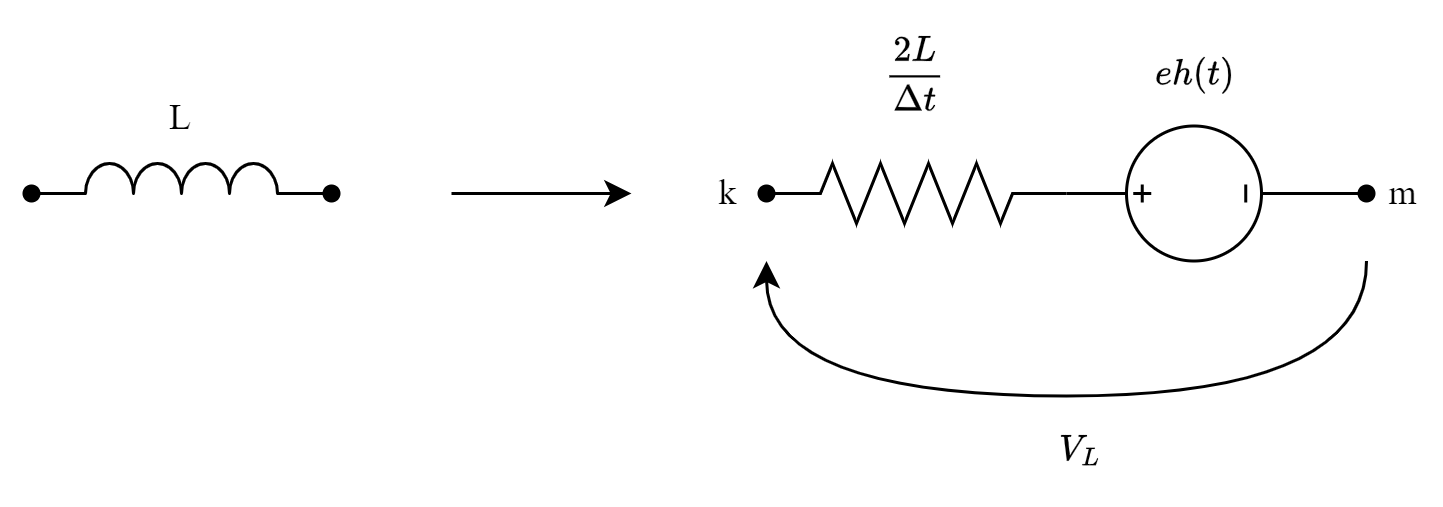
\includegraphics[width = 0.8\columnwidth]{graphics/inductor_discrete.png}
%     \caption{Inductor discrete time equivalent with trapezoidal rule}
%     \label{fig:inductor_discrete}
% \end{figure}

% \section{Discretization Rule Stability} ??????????????????????
\subsection{Nodal Analysis}\label{subsec:ch3/sec5/sub1}
The nodal analysis approach relies on Kirchhoff’s current law, which allows to obtain the voltage in each of the nodes of an electrical circuit. The general form is presented in a simplified form below:
\begin{equation}
    [G][V]=[I]
\end{equation}
where\\  
$G$ represents the $N \times N$ of nodal conductance,\\
$V$ is the vector of nodal voltages,\\  
$I$ are the known vector of current sources injected into the nodes, \\
$N$ is the number of nodes, excluding ground.

The matrix $[G]$ is real, symmetrical and unchanged unless switches or the time step $(\Delta t)$ will change. It is constructed like the nodal admittance matrix used in steady-state analysis. The equations system can be structured using partitioning methods for the nodal conductance matrix and voltage/current vectors:
\begin{equation}
    \left[\begin{array}{ll}
G_{AA} & G_{AB} \\
G_{BA} & G_{BB}
\end{array}\right]\left[\begin{array}{l}
V_{A} \\
V_{B}
\end{array}\right]=\left[\begin{array}{l}
I_{A} \\
I_{B}
\end{array}\right]
\end{equation}
where\\
$V_1$ is the vector of unknown nodal voltages;\\
$V_2$ is the vector of known nodal voltages, in nodes with connected voltage sources.

Then, to find the target node voltages, the Gaussian elimination method is used in the matrix system:
\begin{equation}
    G_{AA} V_{A}=J_{A}-Y_{AB} V_{B}
\end{equation}
Thus, we determine nodal voltages at time $t$, then increase $t$ by $\Delta t$, revise the vector on the right-hand side, and compute nodal voltages, branch voltages, and currents.

\subsection{Discrete Time State-Space Formulation}\label{subsec:ch3/sec5/sub2}
A Linear Time-Invariant (LTI) system can be formulated using discrete-time state-space equations, defined by inputs (external excitations), outputs (measurable quantities), and states (internal dynamics). State variables evolve as functions of past and present states and inputs, so the energy stored in the system at time $t$ is fully determined by the state. A state space representation of a system with multiple inputs and outputs can be visualized in a block diagram, shown in Figure~\cref{fig:ss_block}. 
\begin{figure}[htbp]
    \centering
    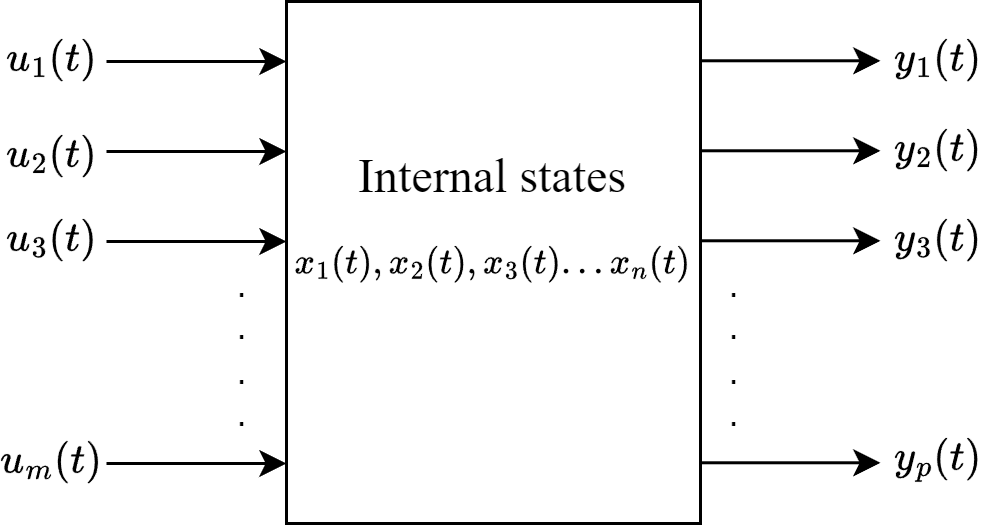
\includegraphics[width = 0.7\columnwidth]{ss_block.png}
    \caption{State-space representation of a multiple input/output system}
    \label{fig:ss_block}
\end{figure}

We consider $m$ inputs, $p$ outputs, and $n$ states. For a system described by $n$ first-order linear difference equations, a minimal state-space representation requires exactly $n$ internal states. At each discrete time instant $t$, the state variables can be expressed as a linear function of the previous state values and the corresponding input values at time $(t - \Delta t)$,
\begin{equation}
    \begin{aligned}
{\left[\begin{array}{c}
x_{1}(t) \\
\vdots \\
x_{n}(t)
\end{array}\right]=} & {\left[\begin{array}{ccc}
a_{11} & \ldots & a_{1 n} \\
\vdots & \ddots & \vdots \\
a_{n 1} & \ldots & a_{n n}
\end{array}\right]\left[\begin{array}{c}
x_{1}(t-\Delta t) \\
\vdots \\
x_{n}(t-\Delta t)
\end{array}\right]+} \\
& {\left[\begin{array}{ccc}
b_{11} & \ldots & b_{1 m} \\
\vdots & \ddots & \vdots \\
a_{n 1} & \ldots & a_{n m}
\end{array}\right]\left[\begin{array}{c}
u_{1}(t-\Delta t) \\
\vdots \\
u_{m}(t-\Delta t)
\end{array}\right] }
\end{aligned}
\label{eq:sv_xau}
\end{equation}

In discrete time $t$, the output variables can be formulated as linear combinations of the input and state variables evaluated at the same instant.
\begin{equation}
    \begin{aligned}
{\left[\begin{array}{c}
y_{1}(t) \\
\vdots \\
y_{p}(t)
\end{array}\right]=} & {\left[\begin{array}{ccc}
c_{11} & \ldots & c_{1 n} \\
\vdots & \ddots & \vdots \\
c_{p 1} & \ldots & c_{p n}
\end{array}\right]\left[\begin{array}{c}
x_{1}(t) \\
\vdots \\
x_{n}(t)
\end{array}\right]+} \\
& {\left[\begin{array}{ccc}
d_{11} & \ldots & d_{1 m} \\
\vdots & \ddots & \vdots \\
d_{p 1} & \ldots & d_{p m n}
\end{array}\right]\left[\begin{array}{c}
u_{1}(t) \\
\vdots \\
u_{m}(t)
\end{array}\right] }
\end{aligned}
\label{eq:sv_ycd}
\end{equation}

For a single input-output system (\ref{eq:sv_xau}) and (\ref{eq:sv_xau}) became
\begin{equation}
    \begin{array}{l}
x(t)=A x(t-\Delta t)+B u(t-\Delta t) \\
y(t)=C x(t)+D u(t)
\end{array}
\end{equation}

The values of a system’s states evolve over time, determined by its memory, the present input, and the structure of its interconnections. State variations may arise from external inputs or from the system’s own internal dynamics. When changes are driven by inputs, they are considered forced, whereas changes produced by internal dynamics reveal the inherent behavior of the system. The simplified state-space diagram, described mentioned interconnections, is presented in Figure~\cref{fig:ss_diagram}.  

\begin{figure}[htbp]
    \centering
    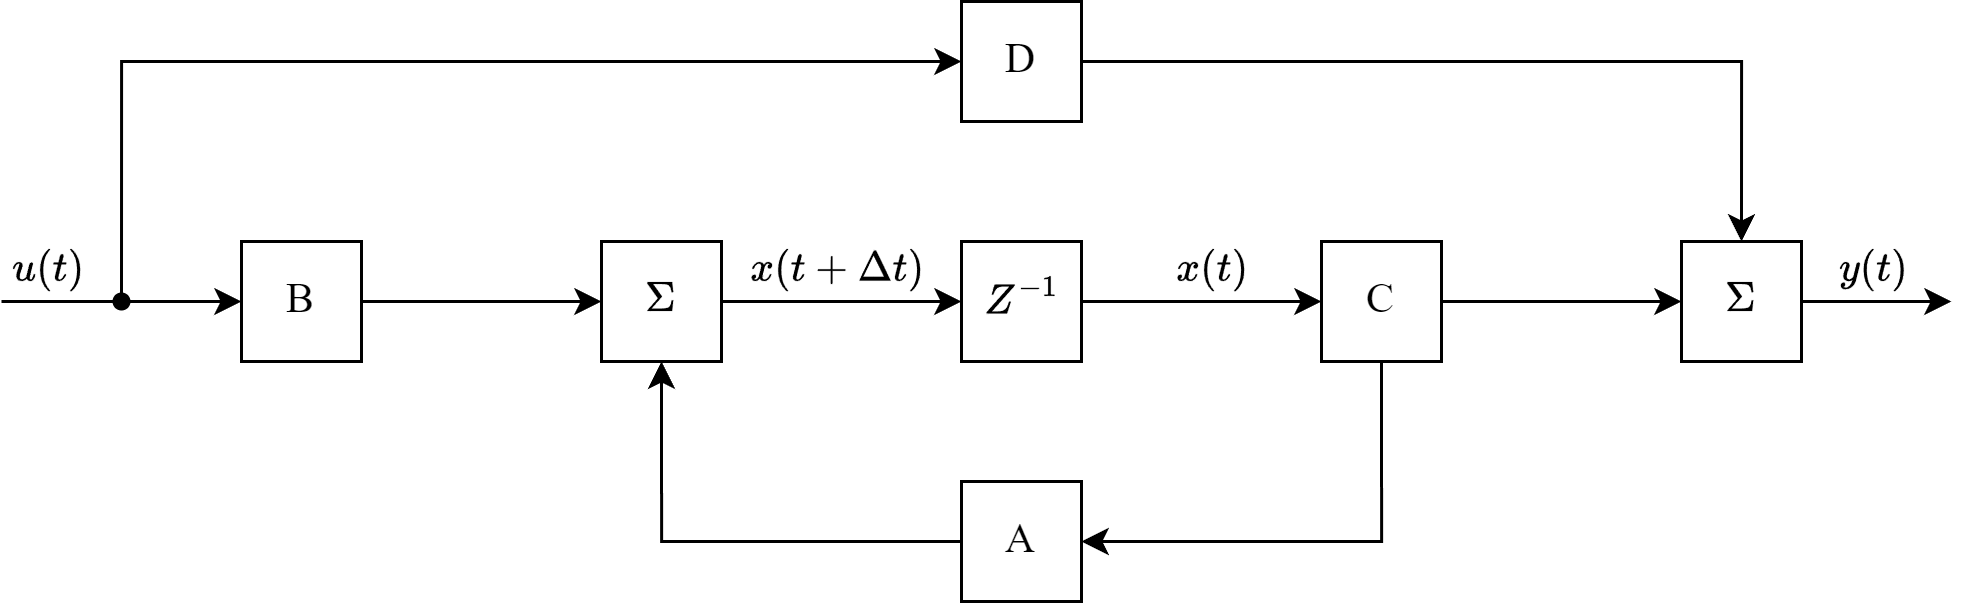
\includegraphics[width = 1\columnwidth]{ss_diagram.png}
    \caption{State-space representation of a multiple input/output system}
    \label{fig:ss_diagram}
\end{figure}

\subsection{EMTP Solution in Discrete Time State-Space form}\label{subsec:ch3/sec5/sub3}
According to the form of the nodal solution for EMTP \autocite{4073845},
\begin{equation}
    [G][v(t)]=[h(t)]+[u(t)]
    \label{eq:ns_emtp}
\end{equation}
Here, $[v(t)]$ denotes the nodal voltages, $[u(t)]$ represents the external current sources, $[G]$ is the nodal conductance matrix, and $[h(t)]$ corresponds to the vector of history sources. The system output can then be written as
\begin{equation}
    [v(t)]=[G]^{-1}[h(t)]+[G]^{-1}[u(t)]
\end{equation}

From historical sources prospective, the equation can be rewritten as
\begin{equation}
    [h(t+\Delta t)]=[A][h(t)]+[B][u(t)]
    \label{eq:ss_hyst}
\end{equation}

As shown, it connects the EMTP solutions with the preceding state idea in the state-space formulation, where the vector $[h(t)]$ represents the history sources as the system memory. This memory combines the system's prior behavior $h(t - \Delta t)$ with the input-influenced dynamics $u(t - \Delta t)$ and aligns well with the state-space definition. The EMTP solution updates $[h(t)]$ in terms of $[h(t - \Delta t)]$  and external current sources (\ref{eq:ss_hyst}), which exactly follows the form (\ref{eq:sv_xau}) of the state-space formulation. This approach describes branch history terms as the states within the electrical network, involving all the necessary information from the EMTP nodal solution and case data input \autocite{rowell1997system}.

\subsection{Discrete Time State-Space Model of the Elements}\label{subsec:ch3/sec5/sub4}
The EMT solution first defines the discretizations at the element level instead of discretizing the entire set of differential equations that describe the behavior of the network \autocite{Linares_Rojas_2001}. Consequently, in the EMT every component relationship between its current and voltage is modeled with a discrete-time equivalent. These difference equations are represented by discrete-time equivalent circuits consisting of resistance and source combinations.

\textbf{Resistance R}. Considering that the resistor is a linear and time-invariant element, the relationship between the voltage at its terminals and the current that flows through it is given by an algebraic equation.
\begin{equation}
    v(t)=Ri(t)
\end{equation}
where
\begin{equation}
    \begin{array}{c}
v(t)=v_{k m}(t)=e_{k}(t)-e_{m}(t), \\
i(t)=i_{k m}(t).
\end{array}
\end{equation}

Thus, the discrete equivalent circuit model of the resistor is itself, as shown in Figure~\cref{fig:emt_r}. In this case $h_{km}(t) = 0$ for all $t$. While resistive components lack branch history and thus do not contribute to the state, they offer damping.

\begin{figure}[htbp]
    \centering
    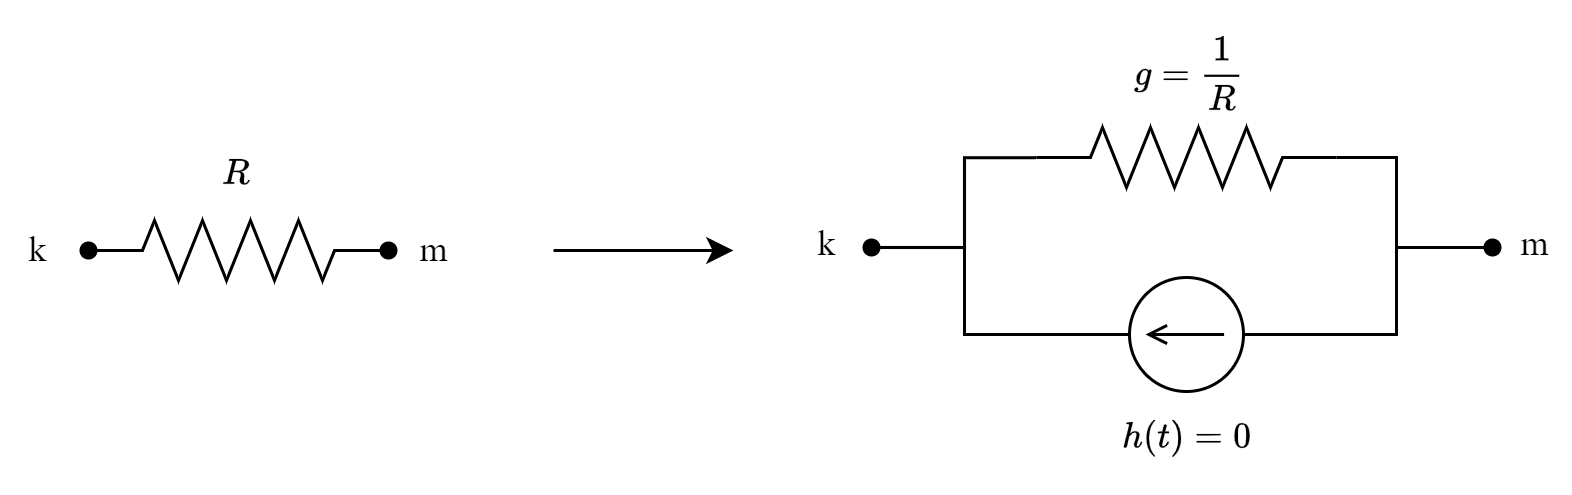
\includegraphics[width = 0.8\columnwidth]{emt_r.png}
    \caption{Discrete equivalent of a resistive element}
    \label{fig:emt_r}
\end{figure}

\textbf{Inductance L}
The discretized inductance is used to model single phase $\pi$-line equivalent, shunt reactors, inductive equivalent parts for loads, and other parts of equivalent circuits. The voltage-current relationship of the element is described by its characteristic equation:
\begin{equation}
    v(t)=L \frac{d i(t)}{d t} .
\end{equation}
Solving for the voltage,
\begin{equation}
\begin{aligned}
    \begin{array}{c}
\displaystyle V_{L} d t=L d i_{L}(t), \\[1em]
\displaystyle \int_{t-\Delta t}^{t} V_{L} d t=L \int_{t-\Delta t}^{t} d i_{L}(t), \\[1em]
\displaystyle \int_{t-\Delta t}^{t} V_{L} d t=L\left[i_{L}(t)-i_{L}(t-\Delta t)\right].
\end{array}
\end{aligned}
\end{equation}
where $\Delta t$ is the discretization time step. Approximating the left-hand side with the trapezoidal formula, we obtain
\begin{equation}
    \frac{V_{L}(t)+V_{L}(t-\Delta t)}{2} \Delta t=L\left[i_{L}(t)-i_{L}(t-\Delta t)\right],
\end{equation}

To obtain the Norton Equivalent Digital Model or the inductor in the discrete time, isolating $i(t)-i(t-\Delta t)$ formula should be converted to:
\begin{equation}
    i(t)-i(\mathrm{t}-\Delta \mathrm{t})=\frac{\Delta t}{2 L} v(t)+\frac{\Delta t}{2 L} v(t-\Delta \mathrm{t}).
\end{equation}
For $i(t)$, we have:
\begin{equation}
    i(t)=\frac{\Delta t}{2 L} v(t)+\frac{\Delta t}{2 L} v(t-\Delta \mathrm{t})+i(t-\Delta t),
\end{equation}
where,
\begin{equation}
    i h_{L}(t)=\left[i(t-\Delta t)+\frac{\Delta t}{2 L} v(t-\Delta t)\right].
    \label{eq:ihl}
\end{equation}

Thus,
\begin{equation}
    i(t)=\frac{\Delta t}{2 L} v(t)+i h_{L}(t).
\end{equation}

To ensure consistent source conversion with the Thévenin Equivalent Digital Model's voltage polarity, the sign in Eq. (\ref{eq:ihl}) giving a form, shown in Figure~\cref{fig:l_eqv2}.
\begin{equation}
\begin{array}{c}
    \displaystyle i h_{L}(t)=\left[-i(t-\Delta t)-\frac{\Delta t}{2 L} v(t-\Delta t)\right],\\[1em]
    \displaystyle i(t)=\frac{\Delta t}{2 L} v(t)-i h_{L}(t).
    \end{array}
\end{equation}

The inductance in Figure~\cref{fig:l_eqv2}'s equivalent circuit represented as a digital resistance $\frac{2 L}{\Delta t}$, paralleled by a historical current source $(ih(t))$, accounting for past data, as it inputs values from prior intervals into the current time step \autocite{de2022introduction}.

\begin{figure}[htbp]
    \centering
    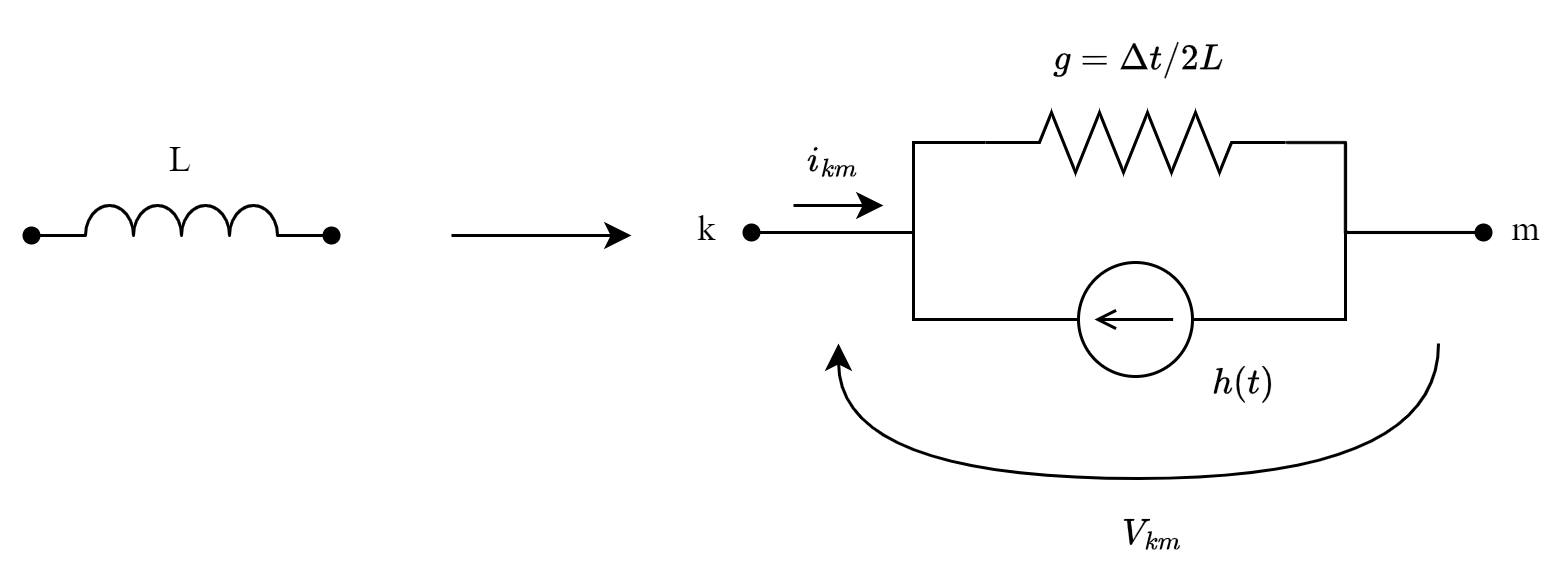
\includegraphics[width = 0.8\columnwidth]{l_eqv2.png}
    \caption{Discrete equivalent of a inductive element}
    \label{fig:l_eqv2}
\end{figure}

\textbf{Capacitance C}. The discretized capacitance generally models series and shunt capacitors in $\pi$-circuit transmission lines, converter parts like filters, capacitance transformers, capacitive dividers, and stray capacitance in generators, particularly for transient recovery voltage and lightning analyzes.

The characteristic equation that outlines the behavior of this element describes the connection between the current flowing through it and the voltage across its terminals:
\begin{equation}
    i(t)=C \frac{d v(t)}{d t}
\end{equation}
Solving for the current,
\begin{equation}
\begin{array}{c}
    \displaystyle i(t) d t=C d v(t),\\[1em]
    \displaystyle \int_{t-\Delta t}^{t} i(\tau) d \tau=C \int_{t-\Delta t}^{t} d v(\tau).
    \label{eq:c_current}
    \end{array}
\end{equation}

Using the trapezoidal rule on Eq. $(\ref{eq:c_current})$ converts the integral-differential form into an algebraic equation, enabling the development of a discrete capacitor model over time as follows:
\begin{equation}
    i(t)=\frac{2 C}{\Delta t} v(t)-i h_{C}(t).
\end{equation}

Thus, we have the Norton Equivalent Digital Model for the capacitor in the discrete time, shown in Figure~\cref{fig:c_eqv}:

\begin{figure}[htbp]
    \centering
    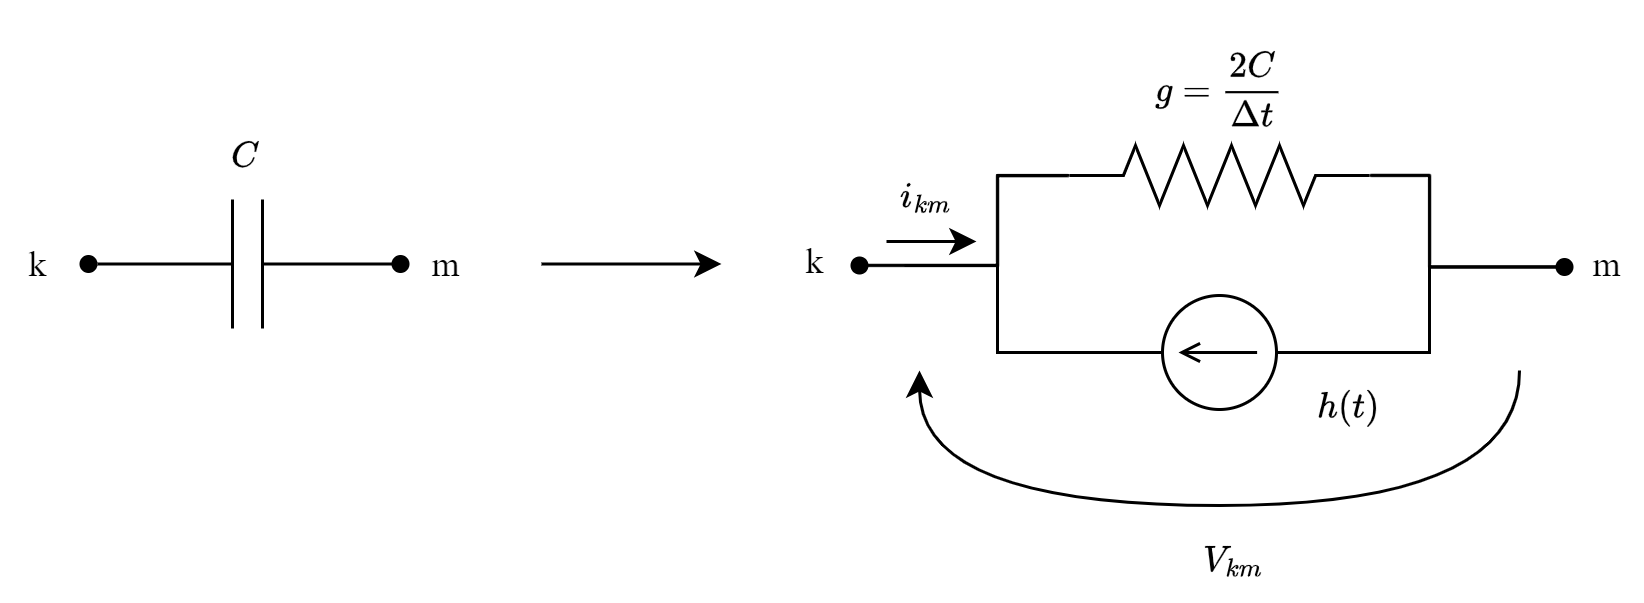
\includegraphics[width = 0.8\columnwidth]{c_eqv.png}
    \caption{Discrete equivalent of a capacitive element}
    \label{fig:c_eqv}
\end{figure}

Observing the equivalent circuit of Figure~\cref{fig:c_eqv}, the capacitance is modeled as an equivalent digital resistance $\Delta t/2C$ alongside a historical current source $(ih(t))$. This source includes past data since it adds values from the prior interval at each new time step.

\textbf{Treatment of Series Connection RL and RC}. The series connection of a resistor and inductor ($RL$) or series pair of resistor and capacitor ($RC$) can be modeled as a single equivalent discrete component. This combined representation accounts for the damping effect of the resistor and enhances computational efficiency by reducing both the number of nodes and branches in the system. The aggregation form of a resistor in series with an inductor is illustrated in Figure~\cref{fig:RL_eqv}.

\begin{figure}[htbp]
    \centering
    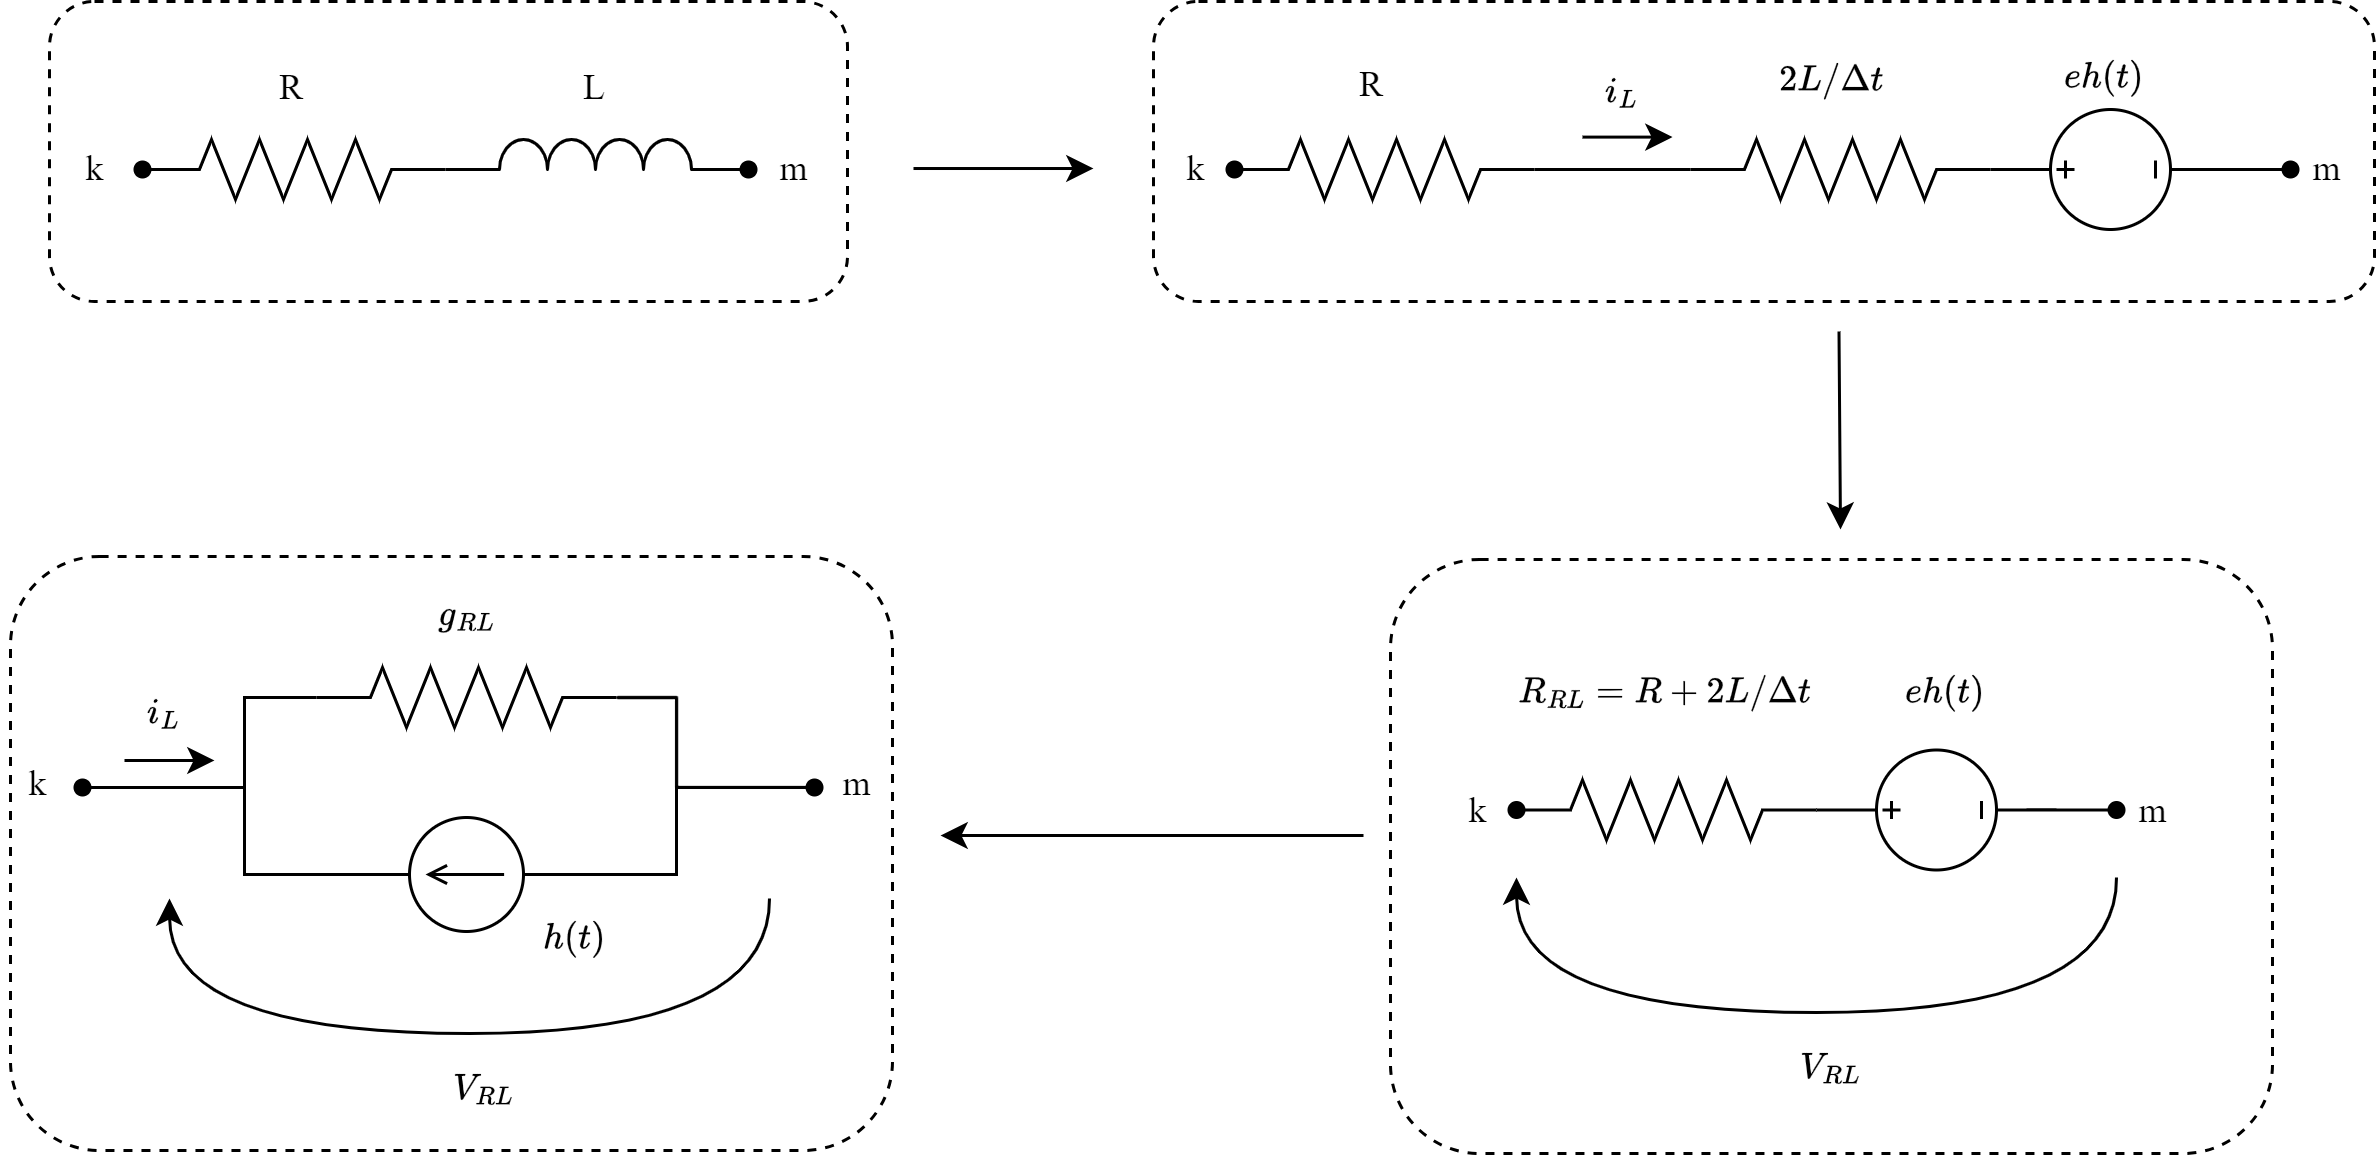
\includegraphics[width = 1\columnwidth]{RL_eqv.png}
    \caption{Discrete equivalent of a capacitive element}
    \label{fig:RL_eqv}
\end{figure}

Here, the connection ($RL$) and ($RC$) is kept respectively, 
\begin{equation}
    \begin{array}{c}
        h_{k m}(t)=h_{k m}(t-\Delta t)-2 g_{R L} v_{k m}(t-\Delta t),\\
        h_{k m}(t)=-h_{k m}(t-\Delta t)+2 g_{R C} v_{k m}(t-\Delta t)
    \end{array}
\end{equation}
where,
\begin{equation}
    g_{R L}=\frac{1}{R+\frac{2 L}{\Delta t}}, \hspace{1em}
    g_{R C}=\frac{1}{R+\frac{\Delta t}{2 C}}
\end{equation}

\textbf{Segmentation of Complex Network}. To provide computational efficiency of the simulation core in real-time for a case with many IBRs connected to the grid, above analysis with EMTP discrete time solutions can be introduced with the Multi-Area Thevenin Equivalent (MATE) concept \autocite{Hollman_2006}. The MATE concept was introduced for handling large power system networks in real-time dynamic studies \autocite{Linares_Rojas_2001, 729230}. The idea is to segment a complex network into independent subnets interconnected by links, as shown in Figure~\cref{fig:mate}. 

\begin{figure}[htbp]
    \centering
    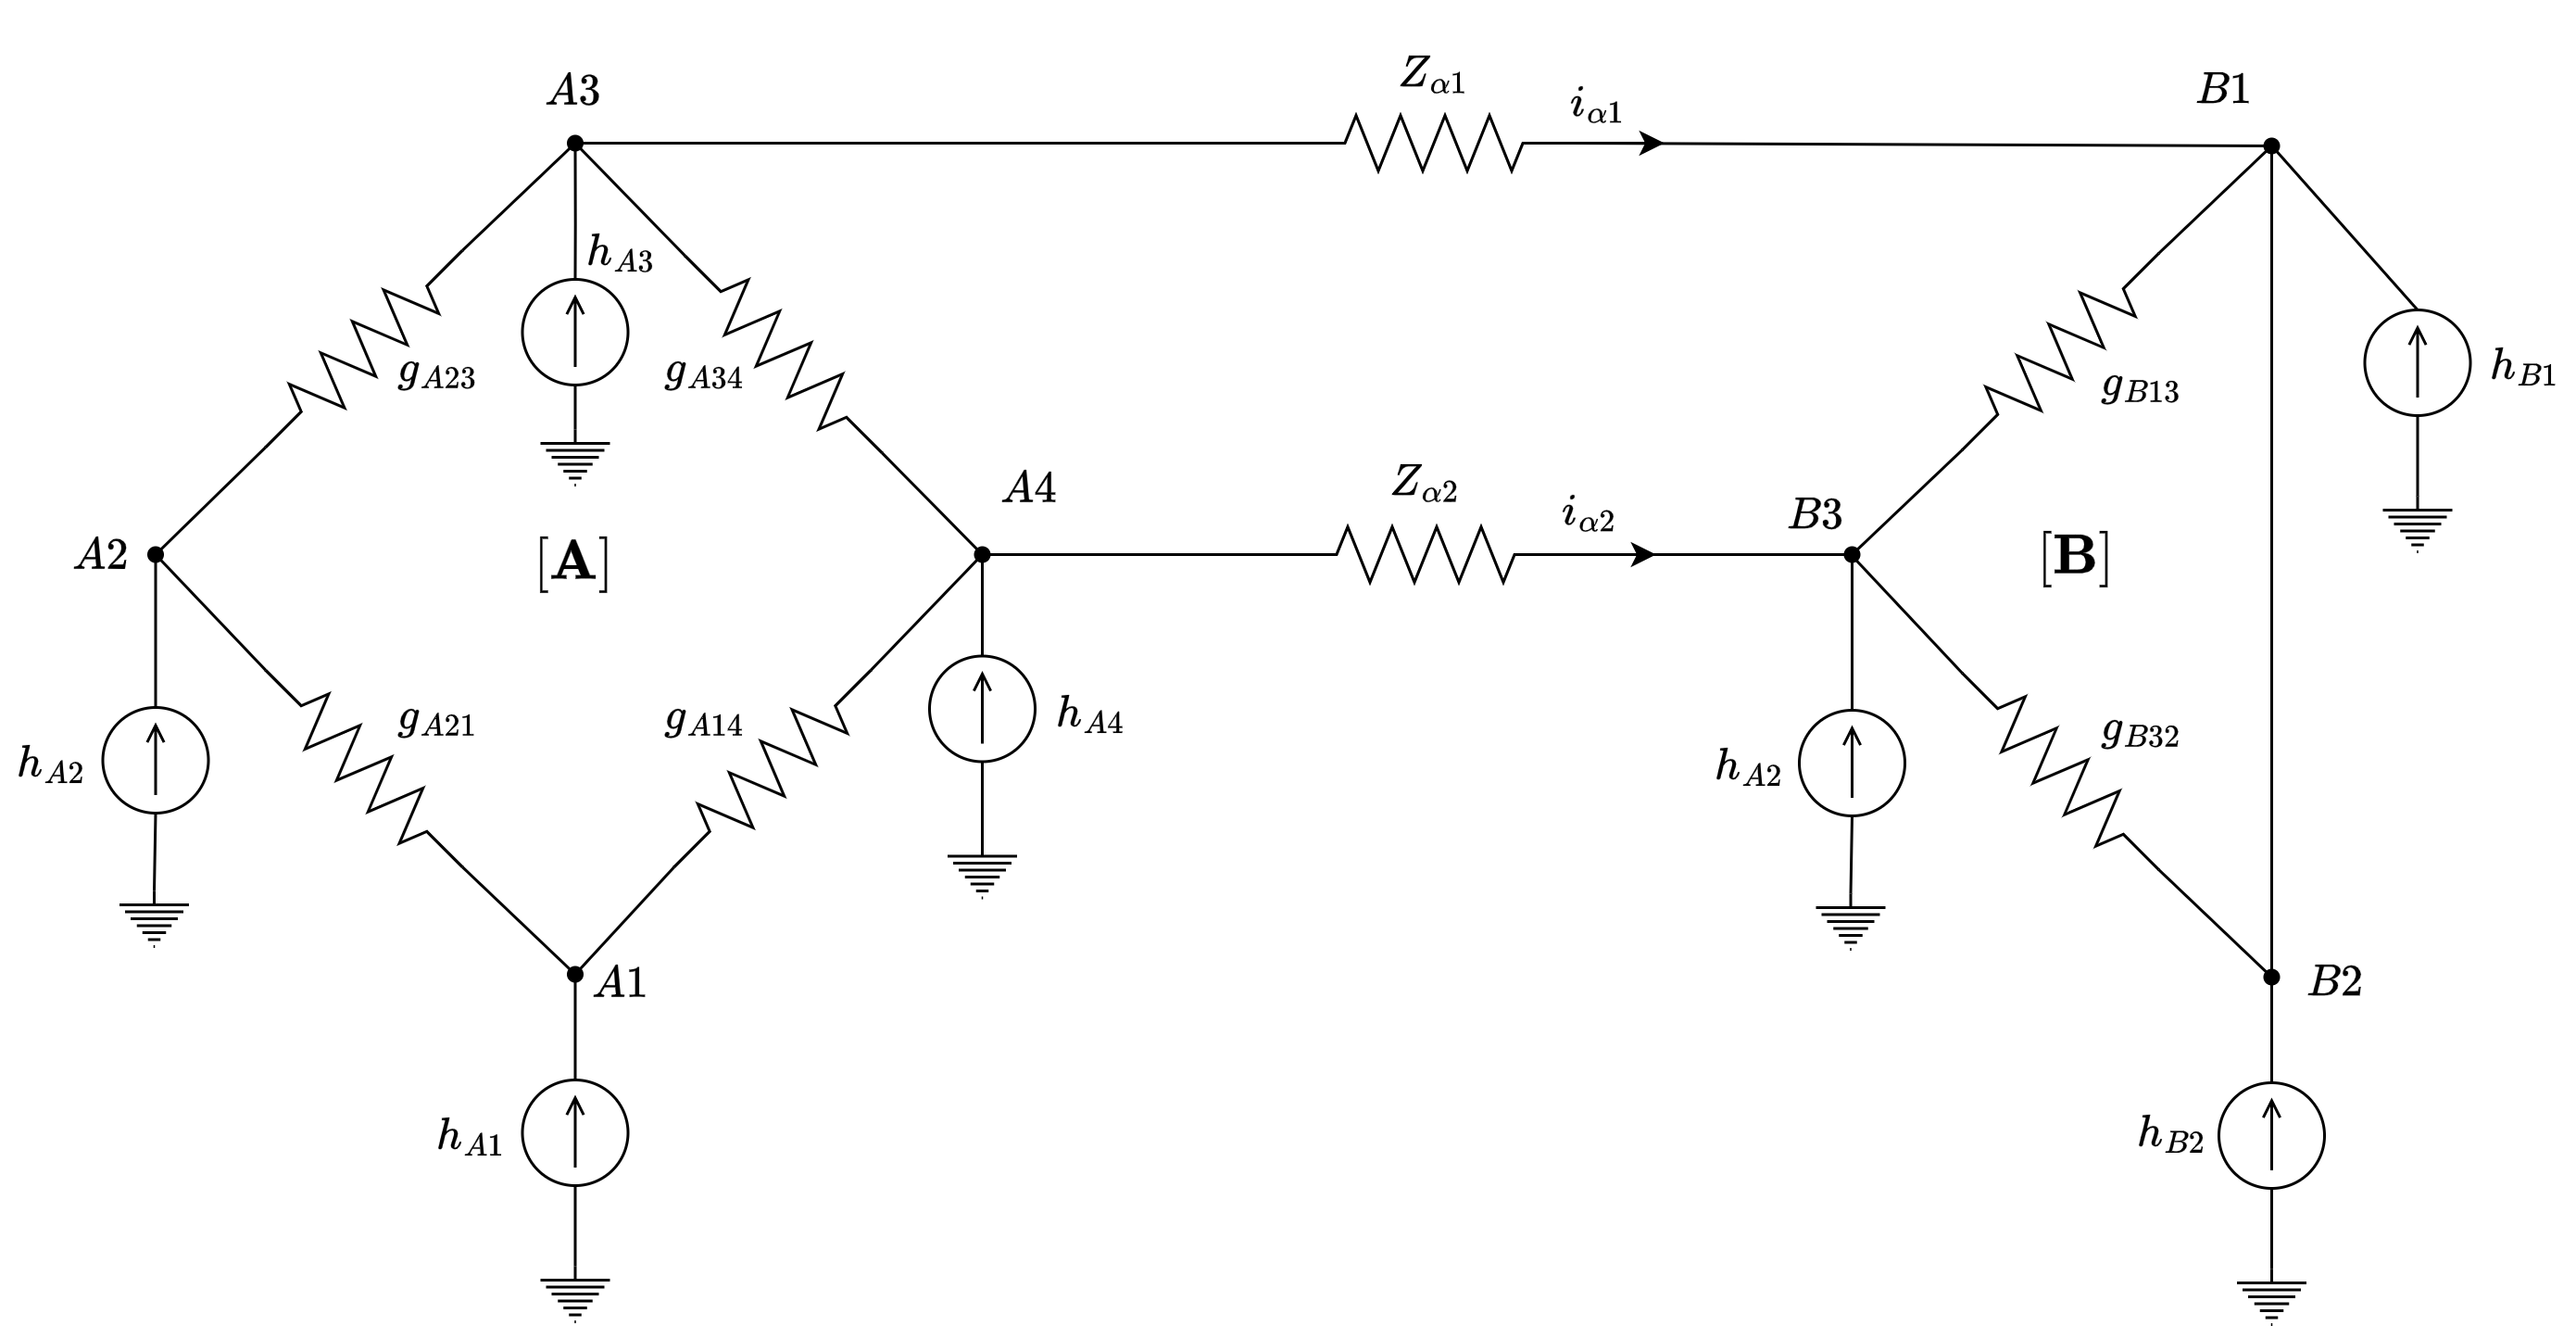
\includegraphics[width = 1\columnwidth]{mate.png}
    \caption{Circuit for discrete state-space MATE explanation \autocite{Mart2002OVNIIS}}
    \label{fig:mate}
\end{figure}

The general nodal equation of the system without the links $\alpha_1$ and $\alpha_2$ is,
\begin{equation}
    \left[\begin{array}{l|l}
A & 0 \\
\hline 0 & B
\end{array}\right]\left[\begin{array}{l}
v_{A} \\
\hline v_{B}
\end{array}\right]=\left[\begin{array}{l}
h_{A} \\
\hline h_{B}
\end{array}\right]
\end{equation}

\setlength{\arraycolsep}{3pt}
\begin{equation}
    \left[\begin{array}{cccc|ccc|cc}
G_{A 11} & G_{A 12} & 0 & G_{A 14} & & & & 0 & 0 \\
G_{A 21} & G_{A 22} & G_{A 23} & & & & & 0 & 0 \\
G_{A 31} & G_{A 32} & G_{A 33} & G_{A 34} & & & & 1 & 0 \\
G_{A 41} & 0 & G_{A 34} & G_{A 44} & & & & 0 & 1 \\
\hline & & & & G_{B 11} & G_{B 12} & G_{B 13} & -1 & 0 \\
& & & & G_{B 21} & G_{B 22} & G_{B 23} & 0 & 0 \\
& & & & G_{B 31} & G_{B 32} & G_{B 33} & 0 & -1 \\
\hline 0 & 0 & 1 & 0 & -1 & 0 & 0 & -z_{1} & 0 \\
0 & 0 & 0 & 1 & 0 & 0 & -1 & 0 & -z_{2}
\end{array}\right]\left[\begin{array}{c}
v_{A 1} \\
v_{A 2} \\
v_{A 3} \\
v_{A 4} \\
\hline v_{B 1} \\
v_{B 2} \\
v_{B 3} \\
\hline i_{\alpha 1} \\
i_{\alpha 2}
\end{array}\right]=\left[\begin{array}{c}
h_{A 1} \\
h_{A 2} \\
h_{A 3} \\
h_{A 4} \\
\hline h_{B 1} \\
h_{B 2} \\
h_{B 3} \\
\hline 0 \\
0
\end{array}\right]
\end{equation}
or it's compact notation,
\begin{equation}
    \left[\begin{array}{c|c|c}
A & 0 & p \\
\hline 0 & B & q \\
\hline p^{t} & q^{t} & -z
\end{array}\right]\left[\begin{array}{c}
v_{A} \\
\hline v_{B} \\
\hline i_{\alpha}
\end{array}\right]=\left[\begin{array}{c}
h_{A} \\
\hline h_{B} \\
\hline 0
\end{array}\right]
\end{equation}
with $[p]$ and $[q]$ as injection matrices from link branches.

This approach divide equivalent circuit into subnetwork nodes, with each node containing necessary information to formulate the discrete state-space equations. All discrete state-space description aggregates by central solver. The process of constructing the discrete state-space formulation of the network can be achieved at once, together with the case preprocessing stage. Only those subnetworks in which there is a topology change have to submit to the central solver the updated discrete state-space formulation \autocite{Hollman_2006}. This is particularly efficient for multicore real-time simulation, since the computation size of the circuit is reduced, as shown in Figure~\cref{fig:mate_mc}.

\begin{figure}[htbp]
    \centering
    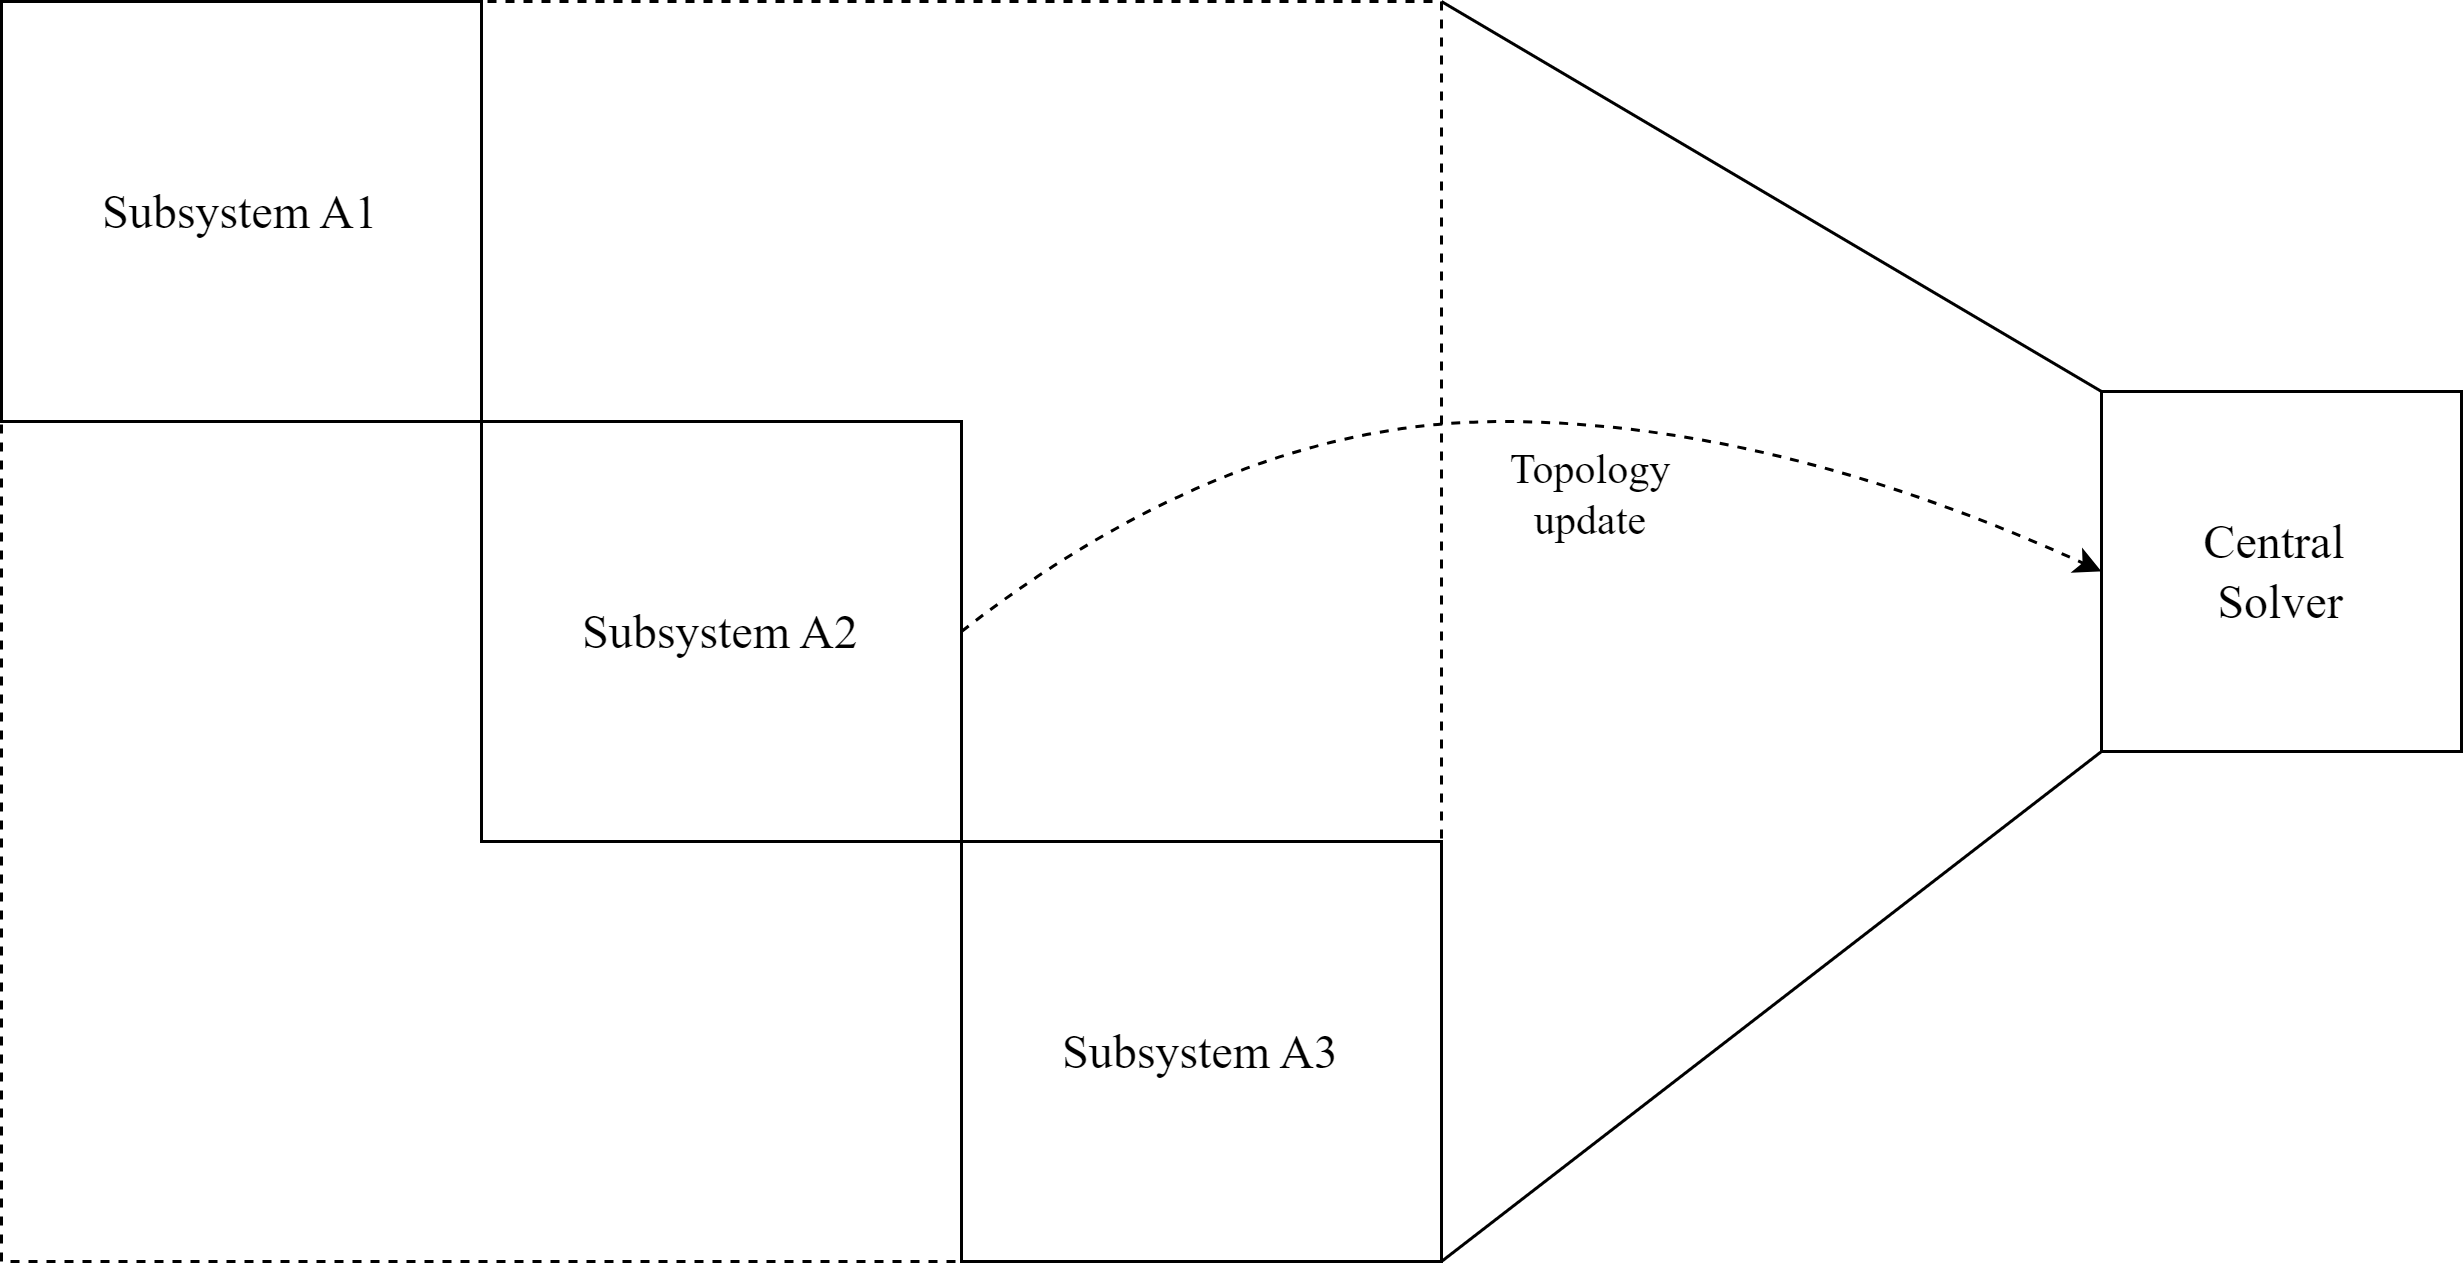
\includegraphics[width = 1\columnwidth]{mate_mc.png}
    \caption{MATE based scheme for multi-core discrete state-space formulation}
    \label{fig:mate_mc}
\end{figure}

To realize such an approach at the hardware level a modern co-simulation concept can be used. A modern co-simulation based approach utilizes the shared memory of computing resources. High-performance shared memory interface can allow multiple processes to directly exchange data with minimal overhead, supported by synchronization mechanisms to ensure consistency at each simulation time step \autocite{Marcus_2021, 8973964}. Simplified scheme of communication, synchronization process, and model interfaces are shown in Figure~\cref{fig:mate_ddm}.

\begin{figure}[htbp]
    \centering
    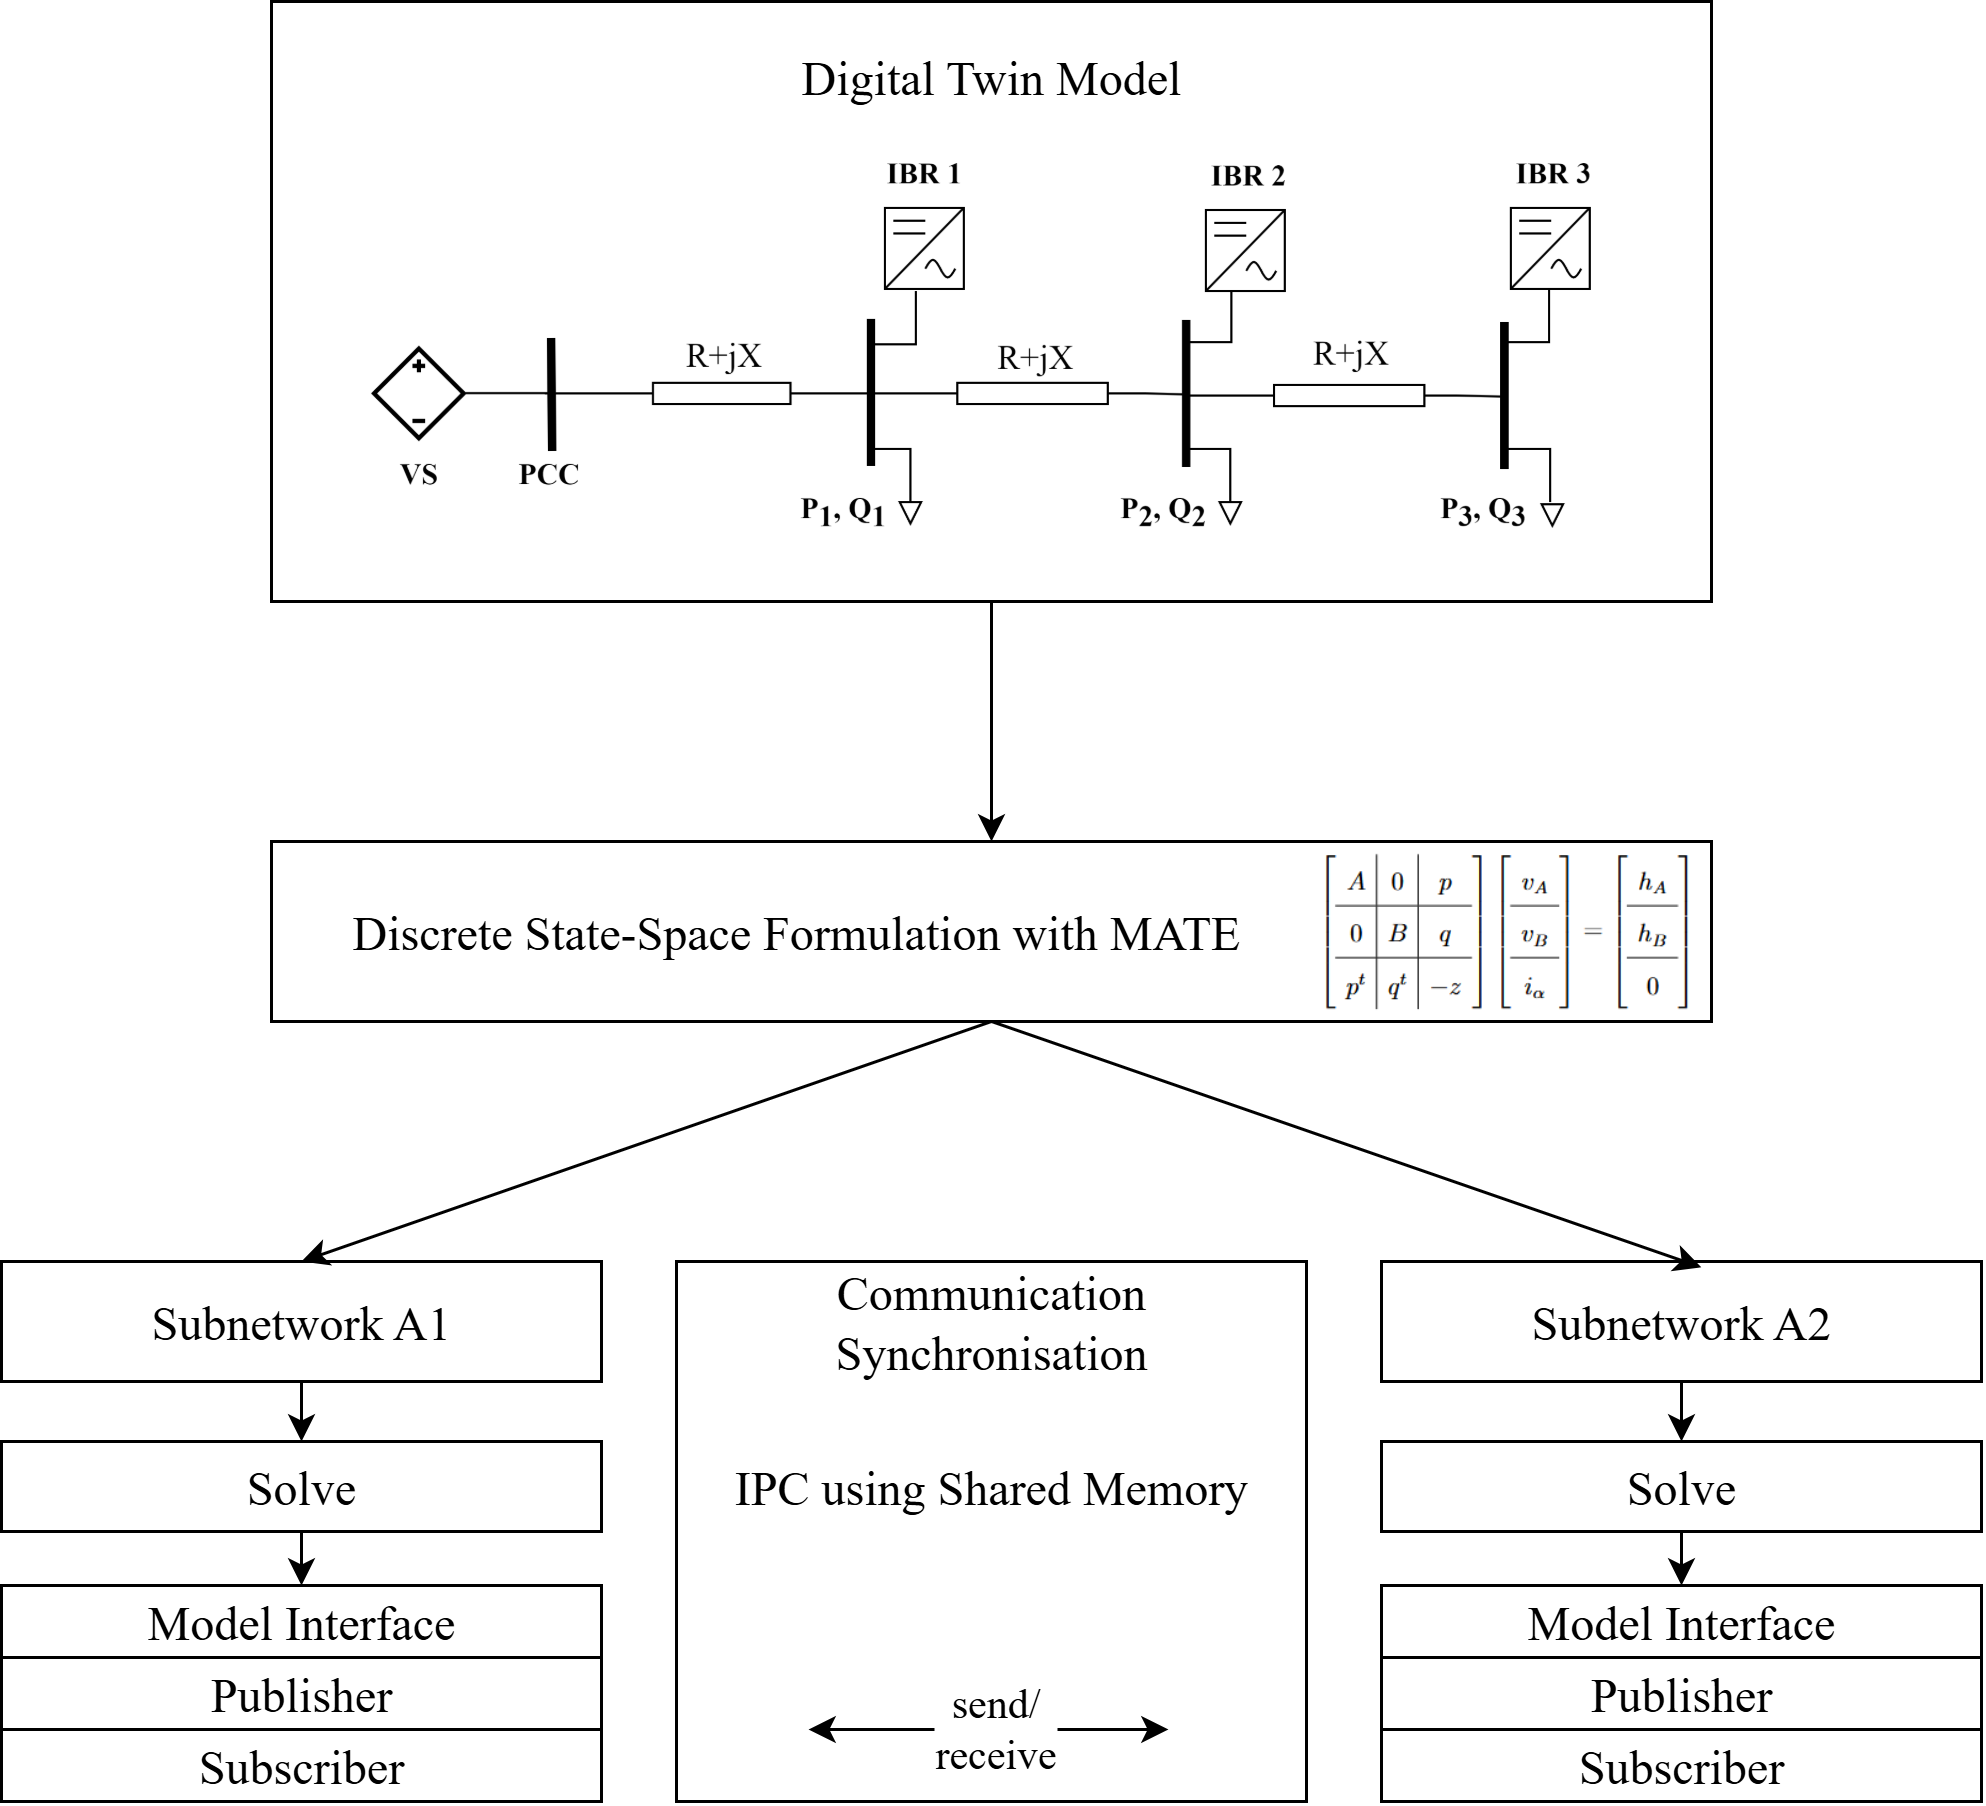
\includegraphics[width = 1\columnwidth]{mate_ddm.png}
    \caption{Concept of digital twin simulation by shared memory parallelization}
    \label{fig:mate_ddm}
\end{figure}


